\section{User interface design}
\label{sect:userinterfacedesign}

TODO: labeling

\subsection{User experience}
\label{subsect:userexperience}

\subsection{Key principles}
\label{subsubsect:keyprinciples}

\noindent
\textbf{Meet the user needs}

The CLup system has relatively few services to offer to the customer and it is therefore essential that the interaction with the views make them stand out. To offer an easy user experience, we want the user to always be able to understand what to do to achieve their goal.

To obtain a result of this type it is essential to identify a hierarchy that is easy to understand.

\noindent
The pages are divided into three levels:
\begin{itemize}[topsep=0pt]
    \item Login and account management Pages;
    \item Home page;
    \item Sub pages: all those pages whose purpose is to guide a user to accomplish a task;
\end{itemize}

The functions of the application, and consequently the paths that a user can take, must also be clearly organized in main flows and sub flows, highlighting and making the most important ones easy to access.

\noindent
\textbf{Consistency}

To facilitate the user experience, consistency is another key factor to consider.

\noindent
Examples of consistency that we will adopt will be:
\begin{itemize}[topsep=0pt]
    \item Colors: to highlight the application brand and make it recognizable and to guide the user.
    \item Interactive colors: to make the user understand that he may or may not interact with a certain element of a graphic interface.
    \item Position of elements: elements with similar goals must always be positioned in key points that characterize them.
    \item Terminology.
    \item Overall view looks.
\end{itemize}

\noindent
\textbf{Less is more}

The "less is more" principle does not mean hiding elements in views, but simply trying not to overload users with information. In general, try to keep the interfaces simple.

This principle is to be particularly kept in mind for pages like the "Home", which has a lot to communicate: it is a gateway for the user to all the main functions, it must be a source of information important events of interest to the user, it must entertain all those users who have no real purpose in mind.

We also use this principle for another very important aspect: the amount of interactions that the user must have with the application. Any page of the application must be easily accessible in a few clicks. The only time we require extra interaction from users is after making a relevant decision: \textit{confirm before commit}.

\noindent
\textbf{Accessibility and demography}

Since the public with which CLup interacts is vast and wide, we try to make stylistic choices as neutral as possible. We do not want to exclude or show particular interest in any demographic group.

In order not to exclude anyone, it is also important to keep in mind possible users with visual impairments.

\subsubsection{Flow diagram}
\label{subsubsect:flowdiagram}

In this section we want to show the flow diagram that represents all the pages in which the application is divided, connected with arrows that indicate how they are reached.

The home page is always the Login Page if the user is not authenticated, otherwise it is the home page.

The image [] represents the flow diagram of the mobile application, it should be read taking into consideration that all the pages on the left are for users, while those on the right are for managers. For the web version, oriented towards PC users, you can use the same diagram, or at most merge some pages together since the space available to work with is greater. The version for the Totem, on the other hand, is a simplified version as many features are not needed.

\begin{figure}[h!]
    \centering
    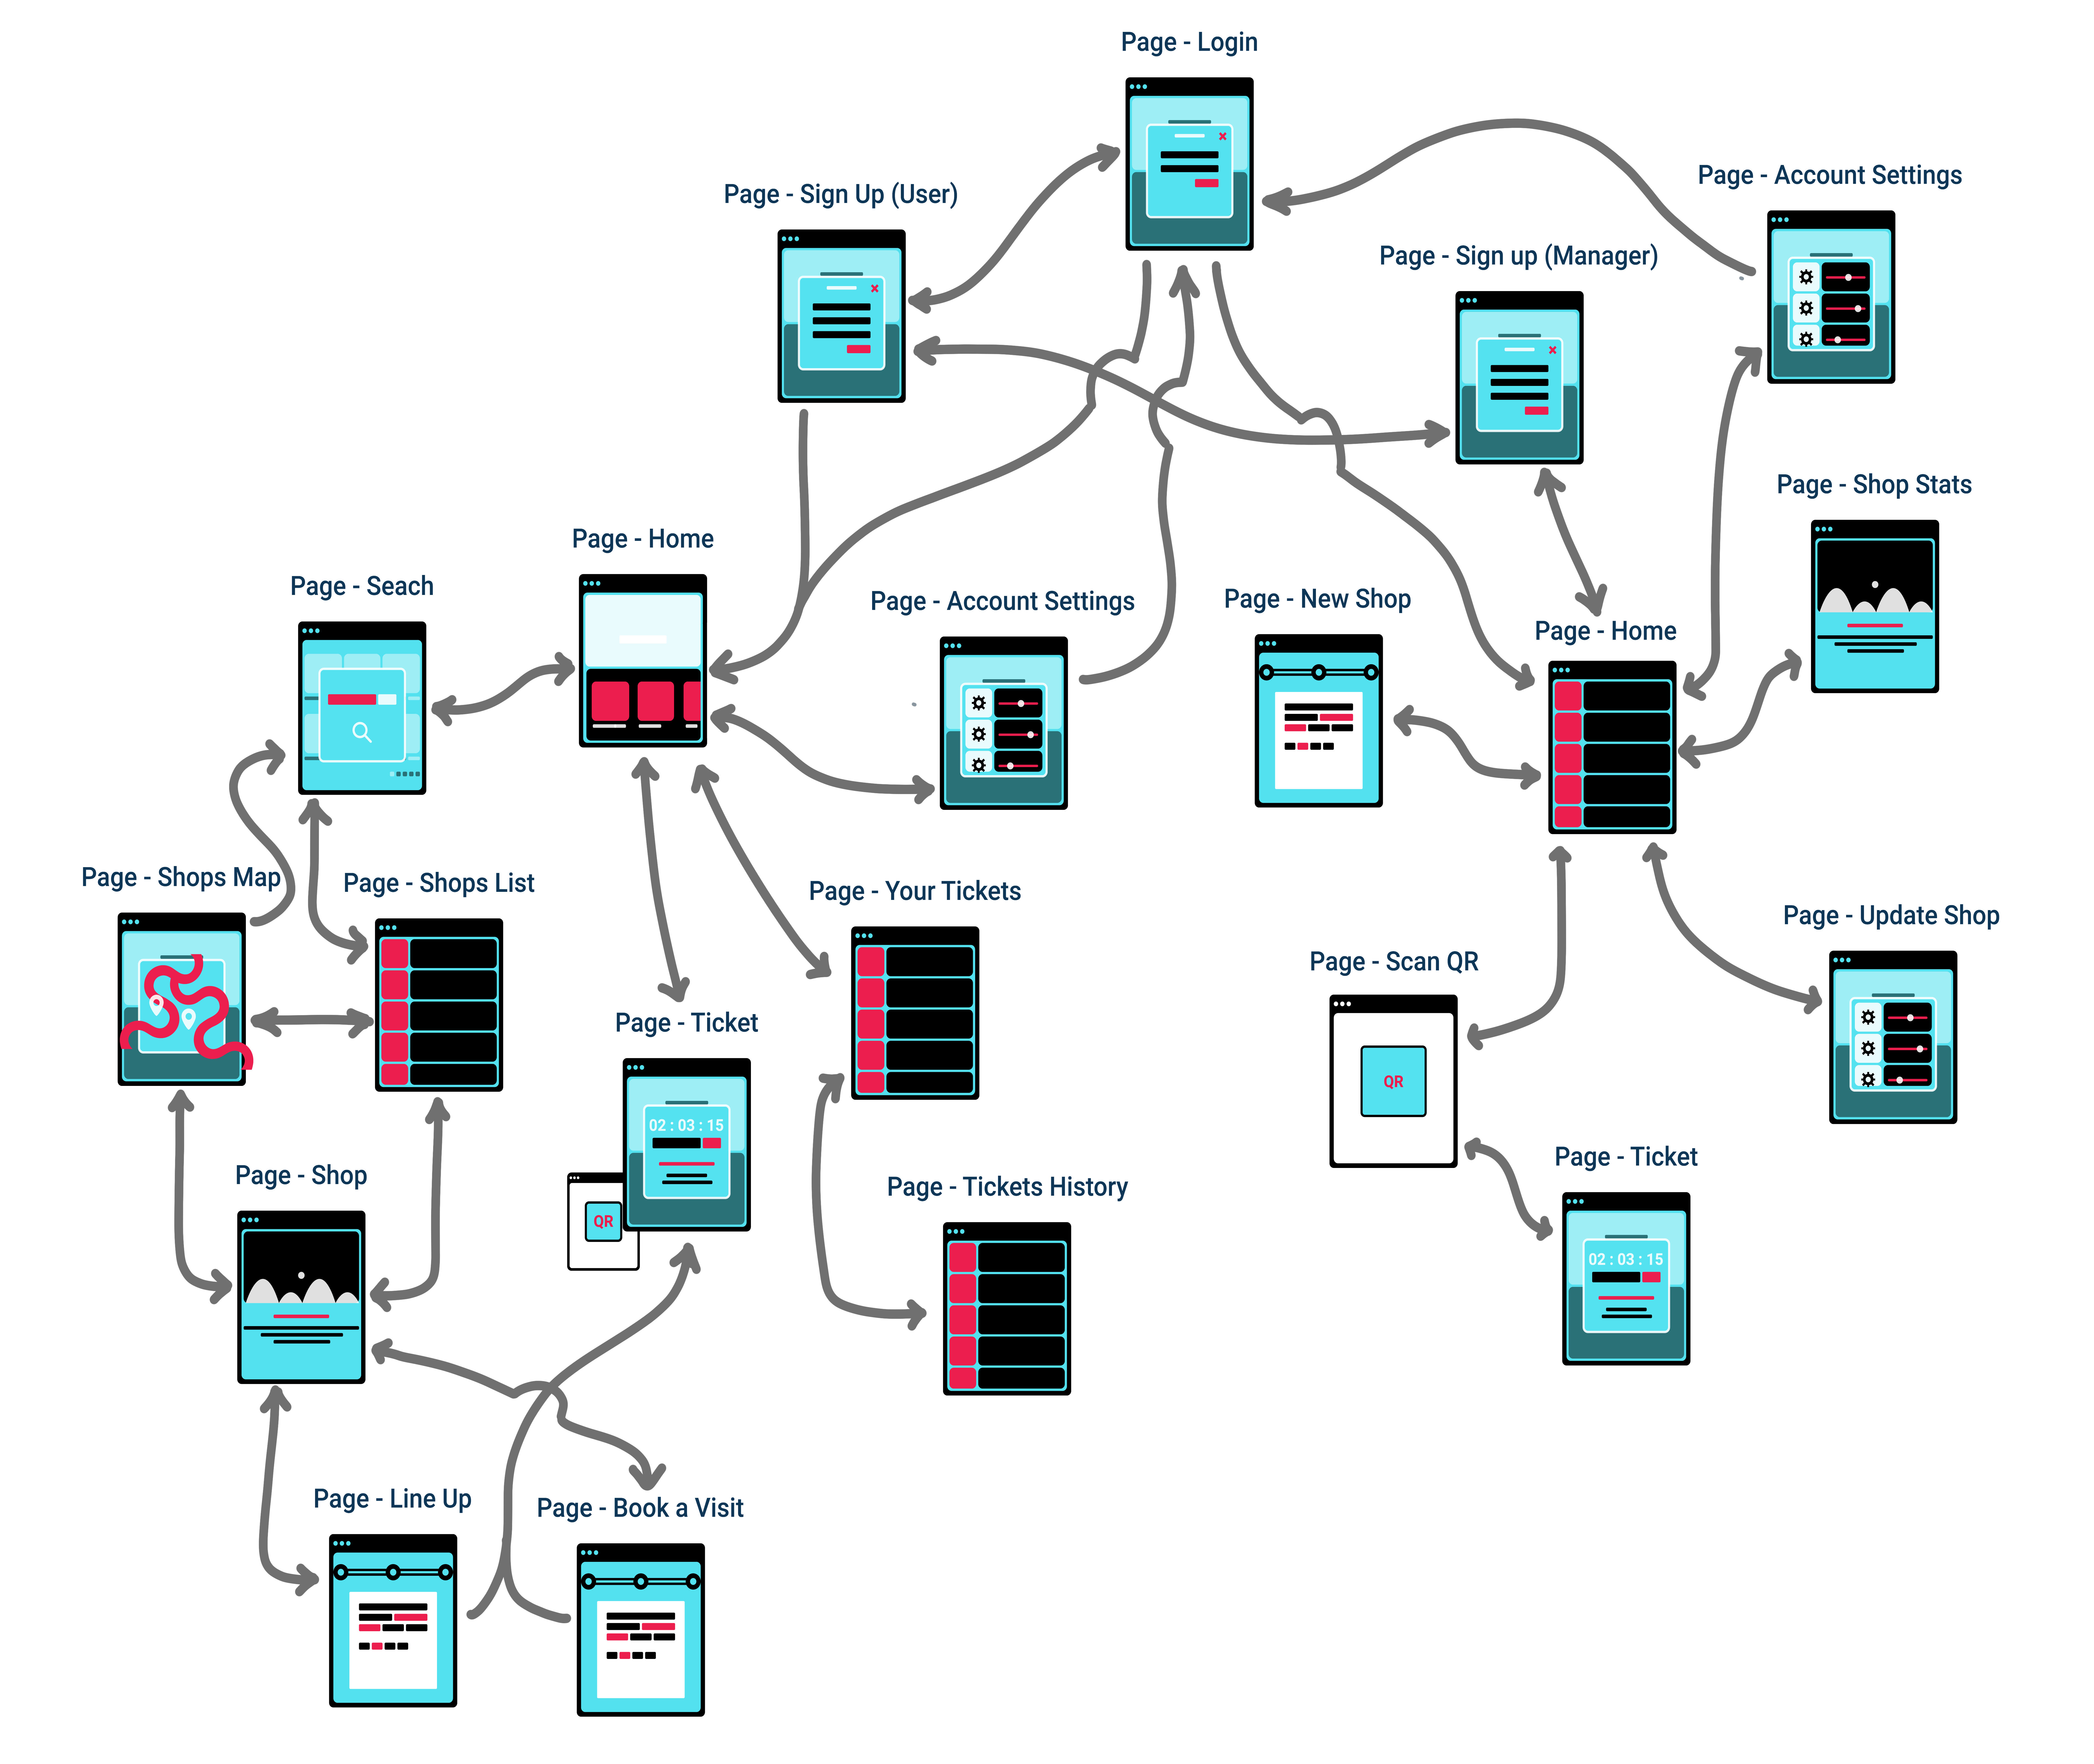
\includegraphics[width=\textwidth]{Images/UserInterfaces/Userinteractions.png}
    \caption{\label{fig:InterfacesDiagram}{Interfaces Diagram}}
\end{figure}

\FloatBarrier

\subsubsection{Views}
\label{subsubsect:Views}

In this section we present some tables that serve to understand the main information of all the pages shown in the image [].

What we want to focus on are the main and secondary functions of each page, as well as some extra informations about the actors that can have access to the pages and some usefull notes.

What we leave out in these tables, however, are the aesthetic details and obvious functionalities, such as error reports, or the elements that allow you to go back to previous views, etc.

Also, it should be noted that each of these pages can be expanded into multiple pages if it can help the user experience.

\begin{table}[h!]
    \centering
    \begin{tabular}{@{}P{0.2\textwidth}P{0.70\textwidth}@{}}
        \multicolumn{2}{c}{\textbf{Login Page}}\\
        \toprule
        \textbf{Main Functions}       & Log in\\
        \textbf{Secondary content}    & -\\
        \textbf{Actors}               & Users and Managers\\
        \textbf{Notes}                & -\\
    \end{tabular}
\caption{Login Page}
\label{table:Login Page}
\end{table}

\begin{table}[h!]
    \centering
    \begin{tabular}{@{}P{0.2\textwidth}P{0.70\textwidth}@{}}
        \multicolumn{2}{c}{\textbf{Sign Up Page}}\\
        \toprule
        \textbf{Main Functions}       & Register\\
        \textbf{Secondary content}    & -\\
        \textbf{Actors}               & Users and Managers\\
        \textbf{Notes}                & Both users and managers have their own page, here they have been merged for simplicity of exposure. Also the page can be split into multiple pages.\\
    \end{tabular}
\caption{Sign Up Page}
\label{table:Sign Up Page}
\end{table}

\begin{table}[h!]
    \centering
    \begin{tabular}{@{}P{0.2\textwidth}P{0.70\textwidth}@{}}
        \multicolumn{2}{c}{\textbf{Account Settings Page}}\\
        \toprule
        \textbf{Main Functions}       & Manage account setting\\
        \textbf{Secondary content}    & Log out\\
        \textbf{Actors}               & Users and Managers\\
        \textbf{Notes}                & Both users and managers have their own page, here they have been merged for simplicity of exposure. Also the page can be split into multiple pages.\\
    \end{tabular}
\caption{Account Settings Page}
\label{table:Account Settings Page}
\end{table}

\begin{table}[h!]
    \centering
    \begin{tabular}{@{}P{0.2\textwidth}P{0.70\textwidth}@{}}
        \multicolumn{2}{c}{\textbf{Home Page (Manager)}}\\
        \toprule
        \textbf{Main Functions}       & Introduce the manager to all possible actions he can take\\
        \textbf{Secondary content}    & -\\
        \textbf{Actors}               & Manager\\
        \textbf{Notes}                & -\\
    \end{tabular}
\caption{Home Page (Manager)}
\label{table:Home Page (Manager)}
\end{table}

\begin{table}[h!]
    \centering
    \begin{tabular}{@{}P{0.2\textwidth}P{0.70\textwidth}@{}}
        \multicolumn{2}{c}{\textbf{Shop Status and Statistics Page}}\\
        \toprule
        \textbf{Main Functions}       & Visualize the current status and the statistics of a shop\\
        \textbf{Secondary content}    & -\\
        \textbf{Actors}               & Manager\\
        \textbf{Notes}                & The page can be split into multiple pages.\\
    \end{tabular}
\caption{Shop Status and Statistics Page}
\label{table:Shop Status and Statistics Page}
\end{table}

\begin{table}[h!]
    \centering
    \begin{tabular}{@{}P{0.2\textwidth}P{0.70\textwidth}@{}}
        \multicolumn{2}{c}{\textbf{New Shop Page}}\\
        \toprule
        \textbf{Main Functions}       & Add a new shop to the system\\
        \textbf{Secondary content}    & -\\
        \textbf{Actors}               & Manager\\
        \textbf{Notes}                & The page can be split into multiple pages.\\
    \end{tabular}
\caption{New Shop Page}
\label{table:New Shop Page}
\end{table}

\begin{table}[h!]
    \centering
    \begin{tabular}{@{}P{0.2\textwidth}P{0.70\textwidth}@{}}
        \multicolumn{2}{c}{\textbf{Update Shop Page}}\\
        \toprule
        \textbf{Main Functions}       & Update shop informations\\
        \textbf{Secondary content}    & -\\
        \textbf{Actors}               & Managers\\
        \textbf{Notes}                & The page can be split into multiple pages.\\
    \end{tabular}
\caption{Update Shop Page}
\label{table:Update Shop Page}
\end{table}

\begin{table}[h!]
    \centering
    \begin{tabular}{@{}P{0.2\textwidth}P{0.70\textwidth}@{}}
        \multicolumn{2}{c}{\textbf{Scan QR-code Page}}\\
        \toprule
        \textbf{Main Functions}       & Identify a ticket easily\\
        \textbf{Secondary content}    & -\\
        \textbf{Actors}               & Managers\\
        \textbf{Notes}                & -\\
    \end{tabular}
\caption{Scan QR-code Page}
\label{table:Scan QR-code Page}
\end{table}

\begin{table}[h!]
    \centering
    \begin{tabular}{@{}P{0.2\textwidth}P{0.70\textwidth}@{}}
        \multicolumn{2}{c}{\textbf{Ticket Page (Manager)}}\\
        \toprule
        \textbf{Main Functions}       & Cancel a ticket from an owned shop queue\\
        \textbf{Secondary content}    & Visualize ticket informations\\
        \textbf{Actors}               & Managers\\
        \textbf{Notes}                & -\\
    \end{tabular}
\caption{Ticket Page (Manager)}
\label{table:Ticket Page (Manager)}
\end{table}

\begin{table}[h!]
    \centering
    \begin{tabular}{@{}P{0.2\textwidth}P{0.70\textwidth}@{}}
        \multicolumn{2}{c}{\textbf{New Shop Page}}\\
        \toprule
        \textbf{Main Functions}       & Add a shop to the system\\
        \textbf{Secondary content}    & -\\
        \textbf{Actors}               & Managers\\
        \textbf{Notes}                & The page can be split into multiple pages.\\
    \end{tabular}
\caption{New Shop Page}
\label{table:New Shop Page}
\end{table}

\begin{table}[h!]
    \centering
    \begin{tabular}{@{}P{0.2\textwidth}P{0.70\textwidth}@{}}
        \multicolumn{2}{c}{\textbf{Home Page (User)}}\\
        \toprule
        \textbf{Main Functions}       & Introduce the user to all possible actions he can take\\
        \textbf{Secondary content}    & Display important events, entertain all those users who have no real purpose in mind.\\
        \textbf{Actors}               & Users\\
        \textbf{Notes}                & -\\
    \end{tabular}
\caption{Home Page (User)}
\label{table:Home Page (User)}
\end{table}

\begin{table}[h!]
    \centering
    \begin{tabular}{@{}P{0.2\textwidth}P{0.70\textwidth}@{}}
        \multicolumn{2}{c}{\textbf{Search Page}}\\
        \toprule
        \textbf{Main Functions}       & Search bar\\
        \textbf{Secondary content}    & Use the device position as the search input\\
        \textbf{Actors}               & Users\\
        \textbf{Notes}                & -\\
    \end{tabular}
\caption{Search Page}
\label{table:Search Page}
\end{table}

\begin{table}[h!]
    \centering
    \begin{tabular}{@{}P{0.2\textwidth}P{0.70\textwidth}@{}}
        \multicolumn{2}{c}{\textbf{Shops List Page}}\\
        \toprule
        \textbf{Main Functions}       & Visualize shops in a list\\
        \textbf{Secondary content}    & Choose a shop, sort the list, filter the list, display basic information for each shop\\
        \textbf{Actors}               & Users\\
        \textbf{Notes}                & -\\
    \end{tabular}
\caption{Shops List Page}
\label{table:Shops List Page}
\end{table}

\begin{table}[h!]
    \centering
    \begin{tabular}{@{}P{0.2\textwidth}P{0.70\textwidth}@{}}
        \multicolumn{2}{c}{\textbf{Shops Map Page}}\\
        \toprule
        \textbf{Main Functions}       & Visualize shops in a map\\
        \textbf{Secondary content}    & Choose a shop, display basic information for each shop\\
        \textbf{Actors}               & Users\\
        \textbf{Notes}                & -\\
    \end{tabular}
\caption{Shops Map Page}
\label{table:Shops Map Page}
\end{table}

\begin{table}[h!]
    \centering
    \begin{tabular}{@{}P{0.2\textwidth}P{0.70\textwidth}@{}}
        \multicolumn{2}{c}{\textbf{Shop Page}}\\
        \toprule
        \textbf{Main Functions}       & Visualize all the information of a shop\\
        \textbf{Secondary content}    & Start the line up and book a visit process\\
        \textbf{Actors}               & Users\\
        \textbf{Notes}                & The page can be split into multiple pages.\\
    \end{tabular}
\caption{Shop Page}
\label{table:Shop Page}
\end{table}

\begin{table}[h!]
    \centering
    \begin{tabular}{@{}P{0.2\textwidth}P{0.70\textwidth}@{}}
        \multicolumn{2}{c}{\textbf{Line Up Page}}\\
        \toprule
        \textbf{Main Functions}       & Line up in a queue\\
        \textbf{Secondary content}    & -\\
        \textbf{Actors}               & Users\\
        \textbf{Notes}                & The page can be split into multiple pages.\\
    \end{tabular}
\caption{Line Up Page}
\label{table:Line Up Page}
\end{table}

\begin{table}[h!]
    \centering
    \begin{tabular}{@{}P{0.2\textwidth}P{0.70\textwidth}@{}}
        \multicolumn{2}{c}{\textbf{Book a visit Page}}\\
        \toprule
        \textbf{Main Functions}       & Book a visit\\
        \textbf{Secondary content}    & -\\
        \textbf{Actors}               & Users\\
        \textbf{Notes}                & The page can be split into multiple pages.\\
    \end{tabular}
\caption{Book a visit Page}
\label{table:Book a visit Page}
\end{table}

\begin{table}[h!]
    \centering
    \begin{tabular}{@{}P{0.2\textwidth}P{0.70\textwidth}@{}}
        \multicolumn{2}{c}{\textbf{Ticket Page (User)}}\\
        \toprule
        \textbf{Main Functions}       & Visualize information about a ticket\\
        \textbf{Secondary content}    & Get the QR-code of a ticket, cancel a ticket\\
        \textbf{Actors}               & Users\\
        \textbf{Notes}                & -\\
    \end{tabular}
\caption{Ticket Page (User)}
\label{table:Ticket Page (User)}
\end{table}

\begin{table}[h!]
    \centering
    \begin{tabular}{@{}P{0.2\textwidth}P{0.70\textwidth}@{}}
        \multicolumn{2}{c}{\textbf{Your Tickets Page}}\\
        \toprule
        \textbf{Main Functions}       & Visualize all active ticket\\
        \textbf{Secondary content}    & -\\
        \textbf{Actors}               & Users\\
        \textbf{Notes}                & -\\
    \end{tabular}
\caption{Your Tickets Page}
\label{table:Your Tickets Page}
\end{table}

\begin{table}[h!]
    \centering
    \begin{tabular}{@{}P{0.2\textwidth}P{0.70\textwidth}@{}}
        \multicolumn{2}{c}{\textbf{Ticket History Page}}\\
        \toprule
        \textbf{Main Functions}       & Visualize all past tickets\\
        \textbf{Secondary content}    & -\\
        \textbf{Actors}               & Users\\
        \textbf{Notes}                & -\\
    \end{tabular}
\caption{Ticket History Page}
\label{table:Ticket History Page}
\end{table}

\FloatBarrier

\subsection{User interfaces}
\label{subsect:mockups}

\subsubsection{Colors}
\label{subsubsect:colors}

\begin{figure}[h!]
    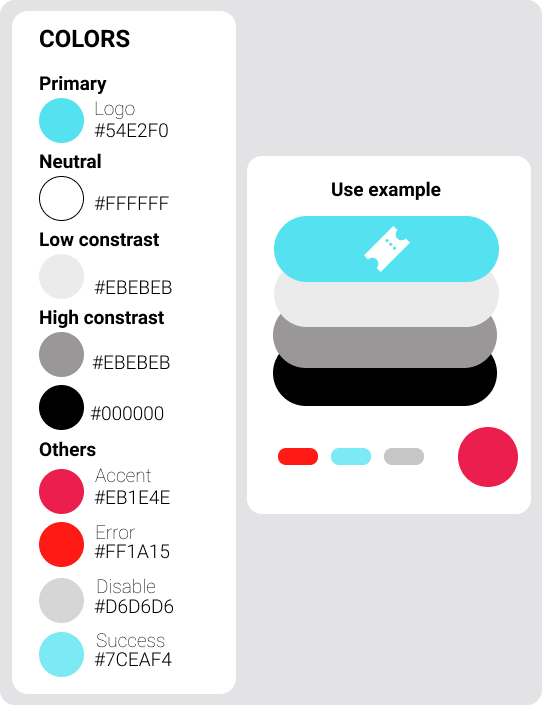
\includegraphics[width=0.5\textwidth]{Images/UserInterfaces/colors.png}
    \caption{\label{fig:InterfacesDiagram}{Colors palette}}
\end{figure}

\FloatBarrier

\noindent
We present the chosen colors:

\begin{itemize}[topsep=0pt]
    \item Company color: \#54E2F0. This color should be used throughout the application to make the CLup brand stand out and to make it recognized outside the system.
    \item Accent color: \#EB1E4E. This color should be used throughout the application to communicate to the users what elements they can interact with.
    \item Error color: \#FF1A15. This color should be used to highlight errors.
    \item Disable color: \#D6D6D6. This color should be used to highlight disabled element.
    \item Success color: \#7CEAF4. This color should be used to highlight a successful operation.
\end{itemize}

\subsubsection{Mockups}
\label{subsubsect:mockups}

In this section we show experimental mockups for some pages of the CLup mobile application.

\begin{figure}
    \centering
    \begin{minipage}{.45\linewidth}
    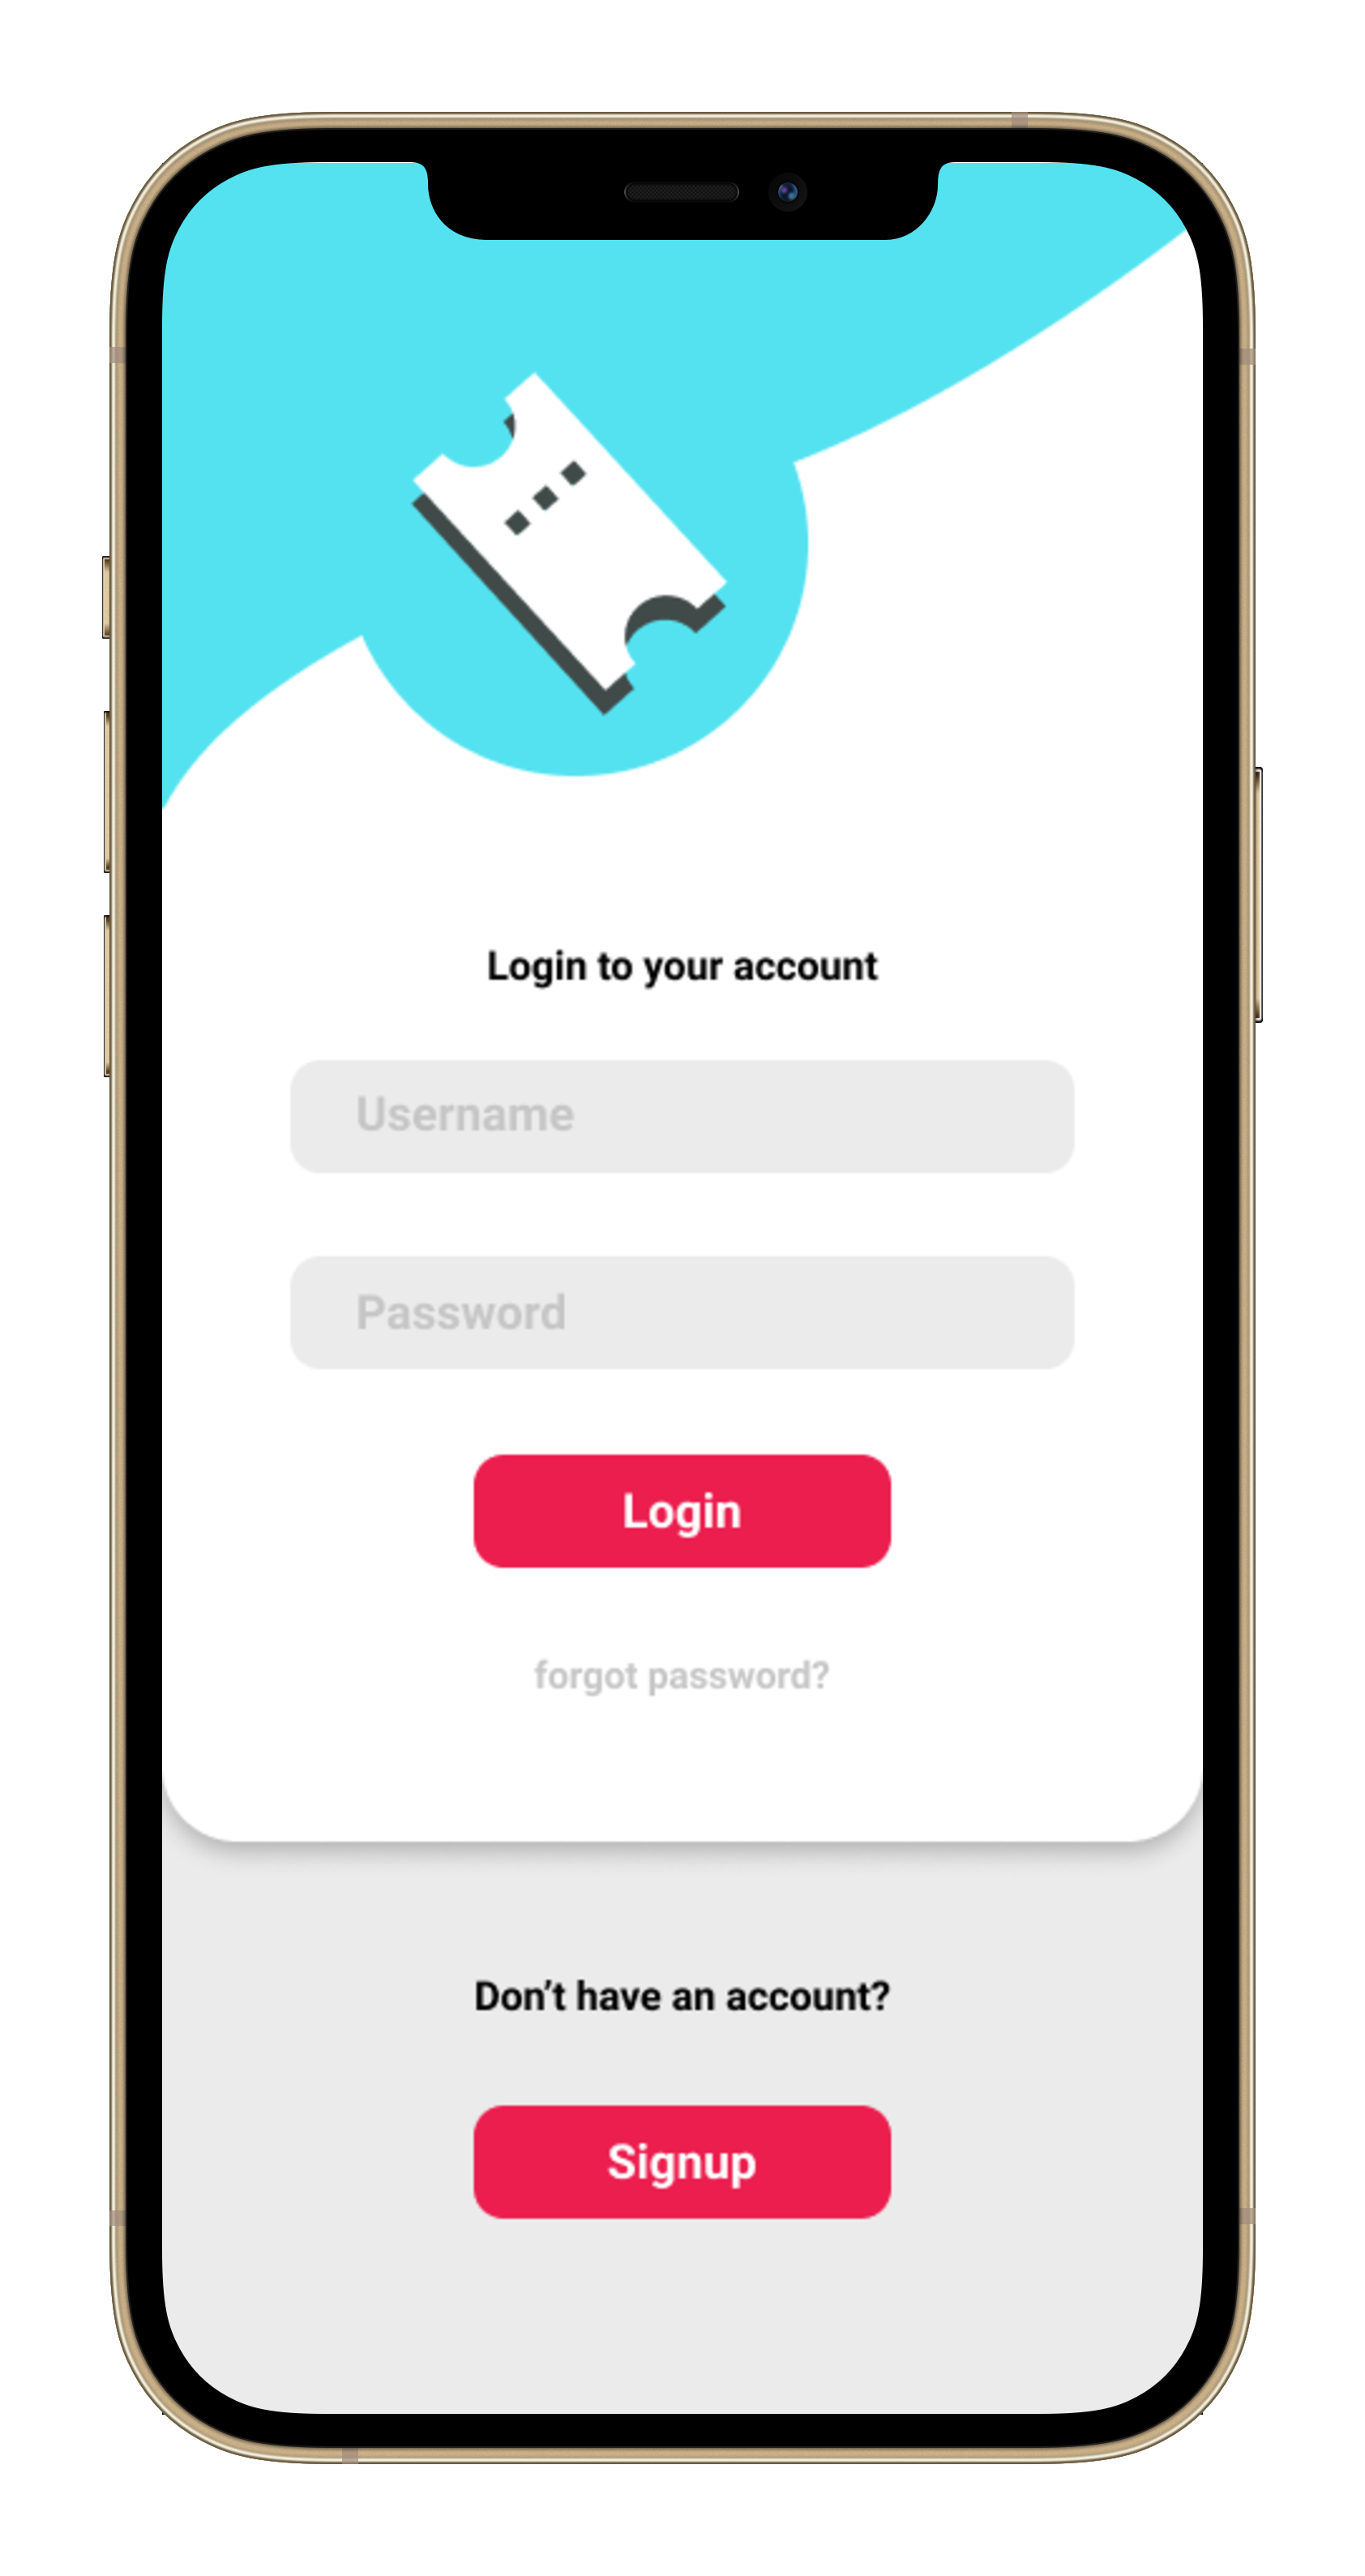
\includegraphics[width=0.9\textwidth]{Images/UserInterfaces/withiphonephrames/LoginPage_iphone12promaxgold_portrait.png}
    \caption{\label{fig:InterfacesDiagram}{Login Page Mockup}}
\end{minipage}
\hspace{.05\linewidth}
\begin{minipage}{.45\linewidth}
    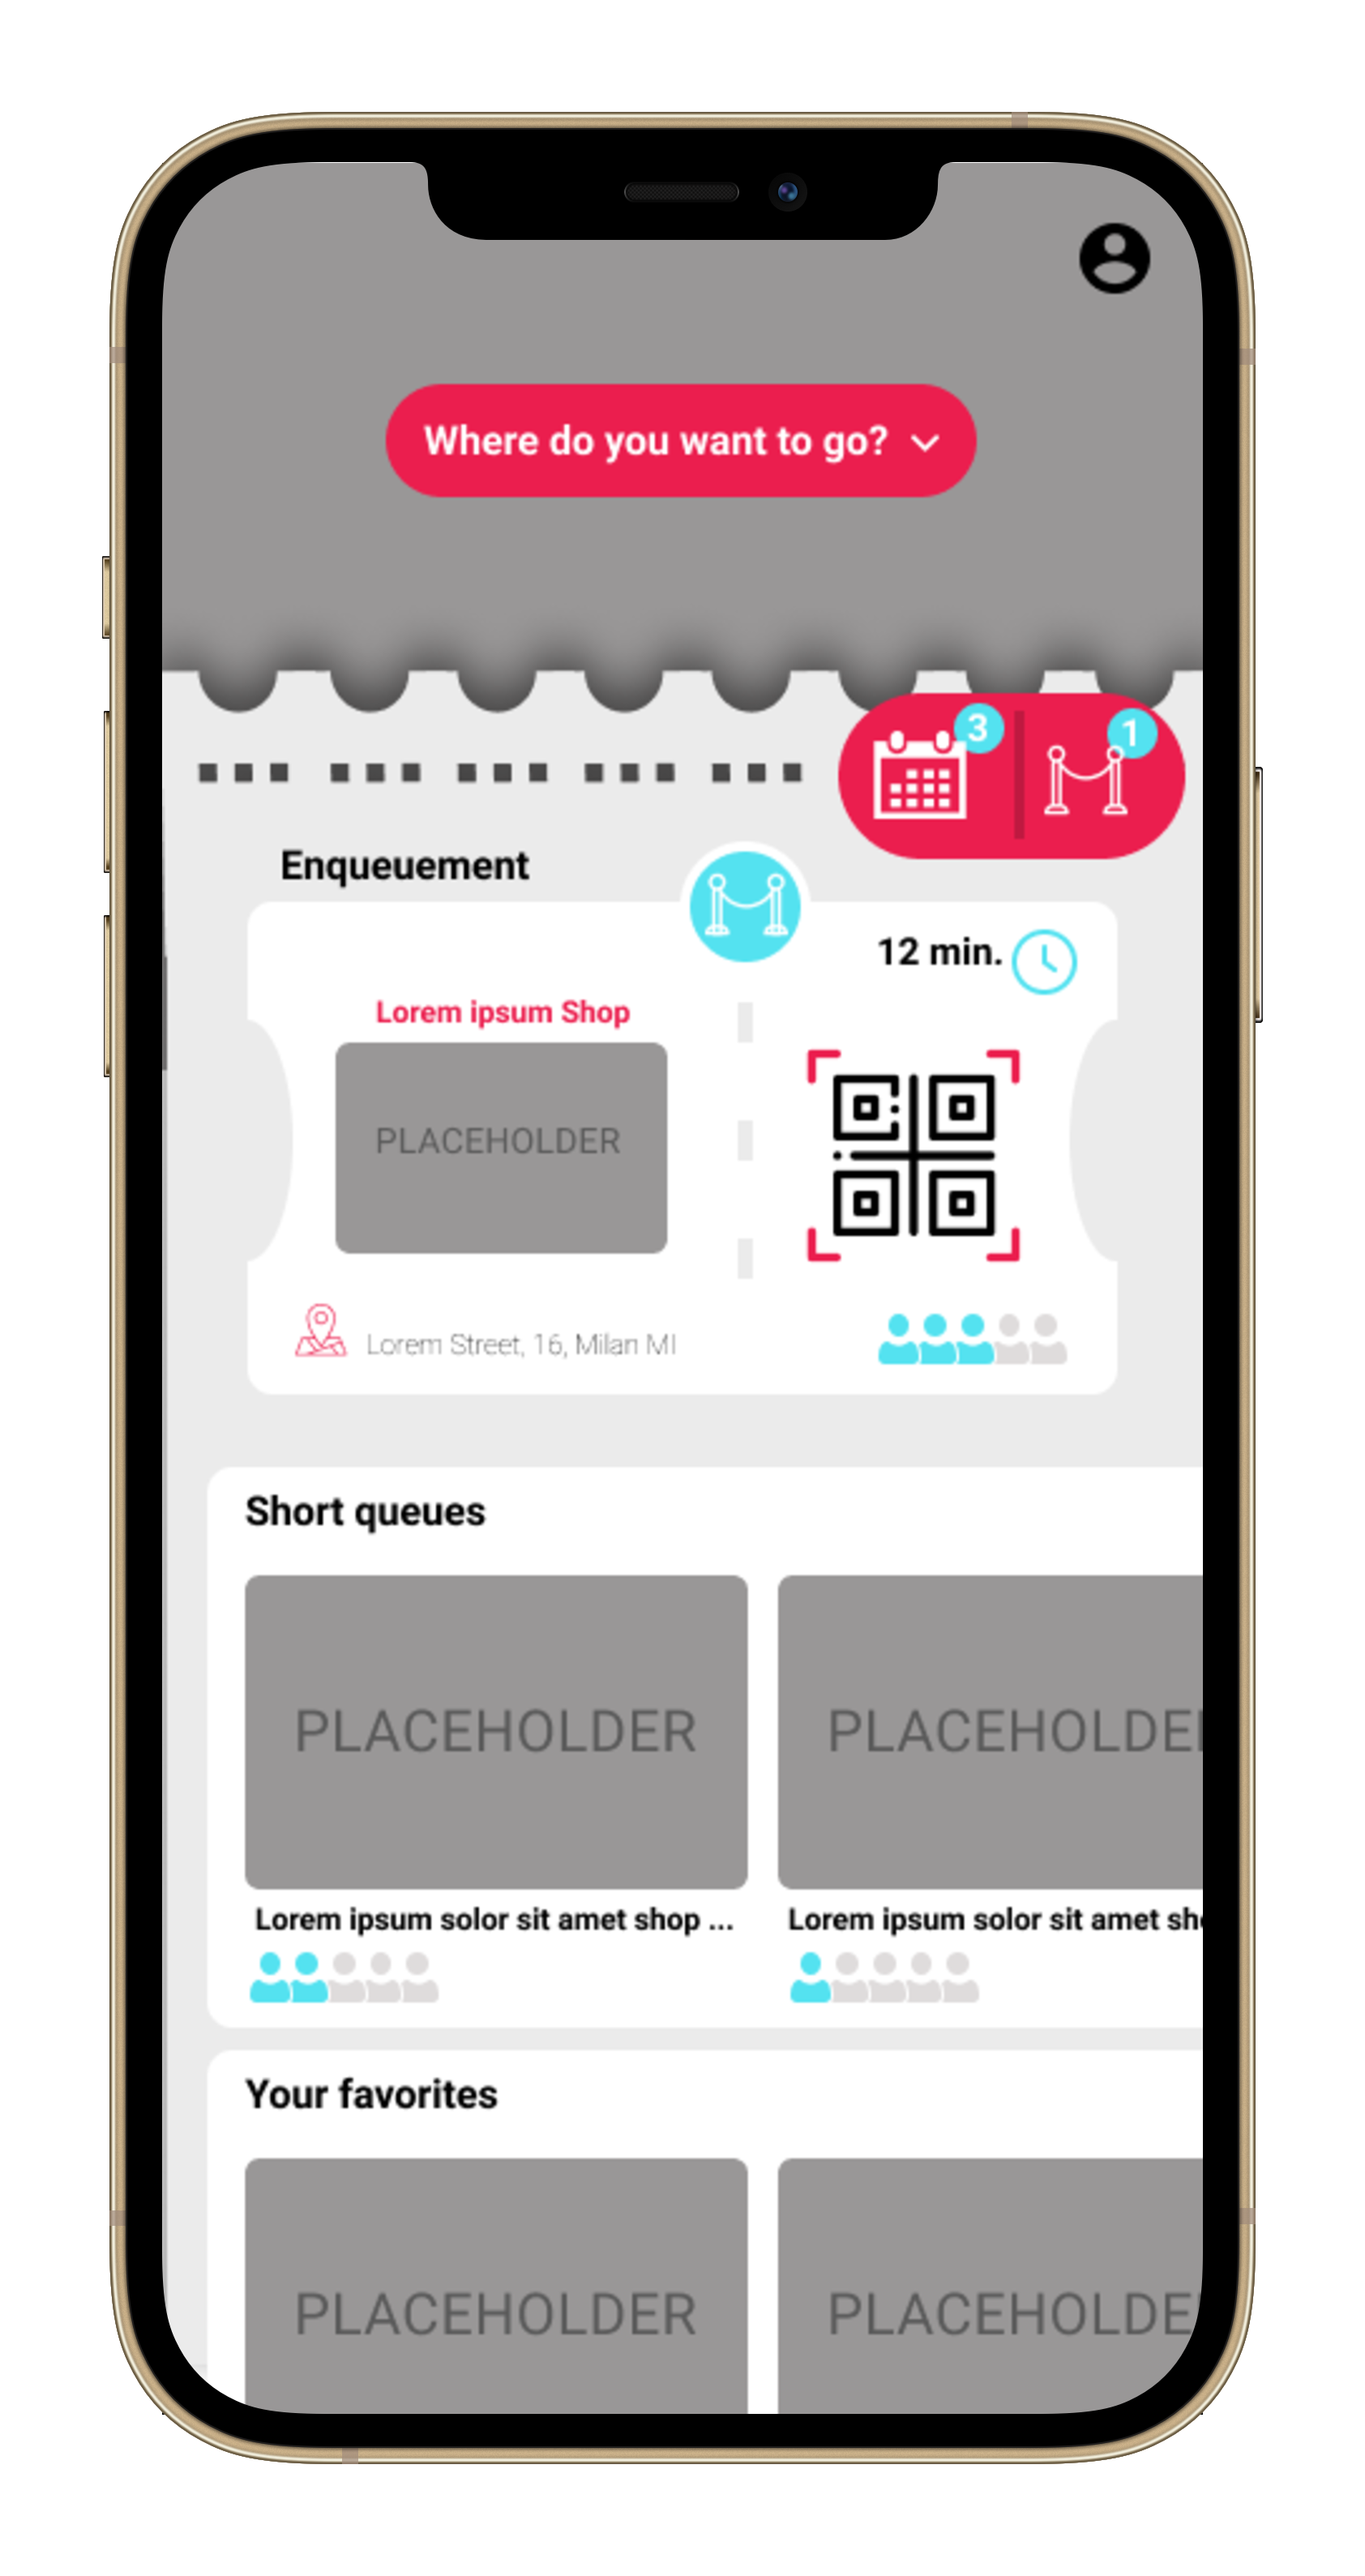
\includegraphics[width=0.9\textwidth]{Images/UserInterfaces/withiphonephrames/HomePage_iphone12promaxgold_portrait.png}
    \caption{\label{fig:InterfacesDiagram}{User Home Page Mockup}}
\end{minipage}
\end{figure}

\begin{figure}
    \centering
    \begin{minipage}{.45\linewidth}
    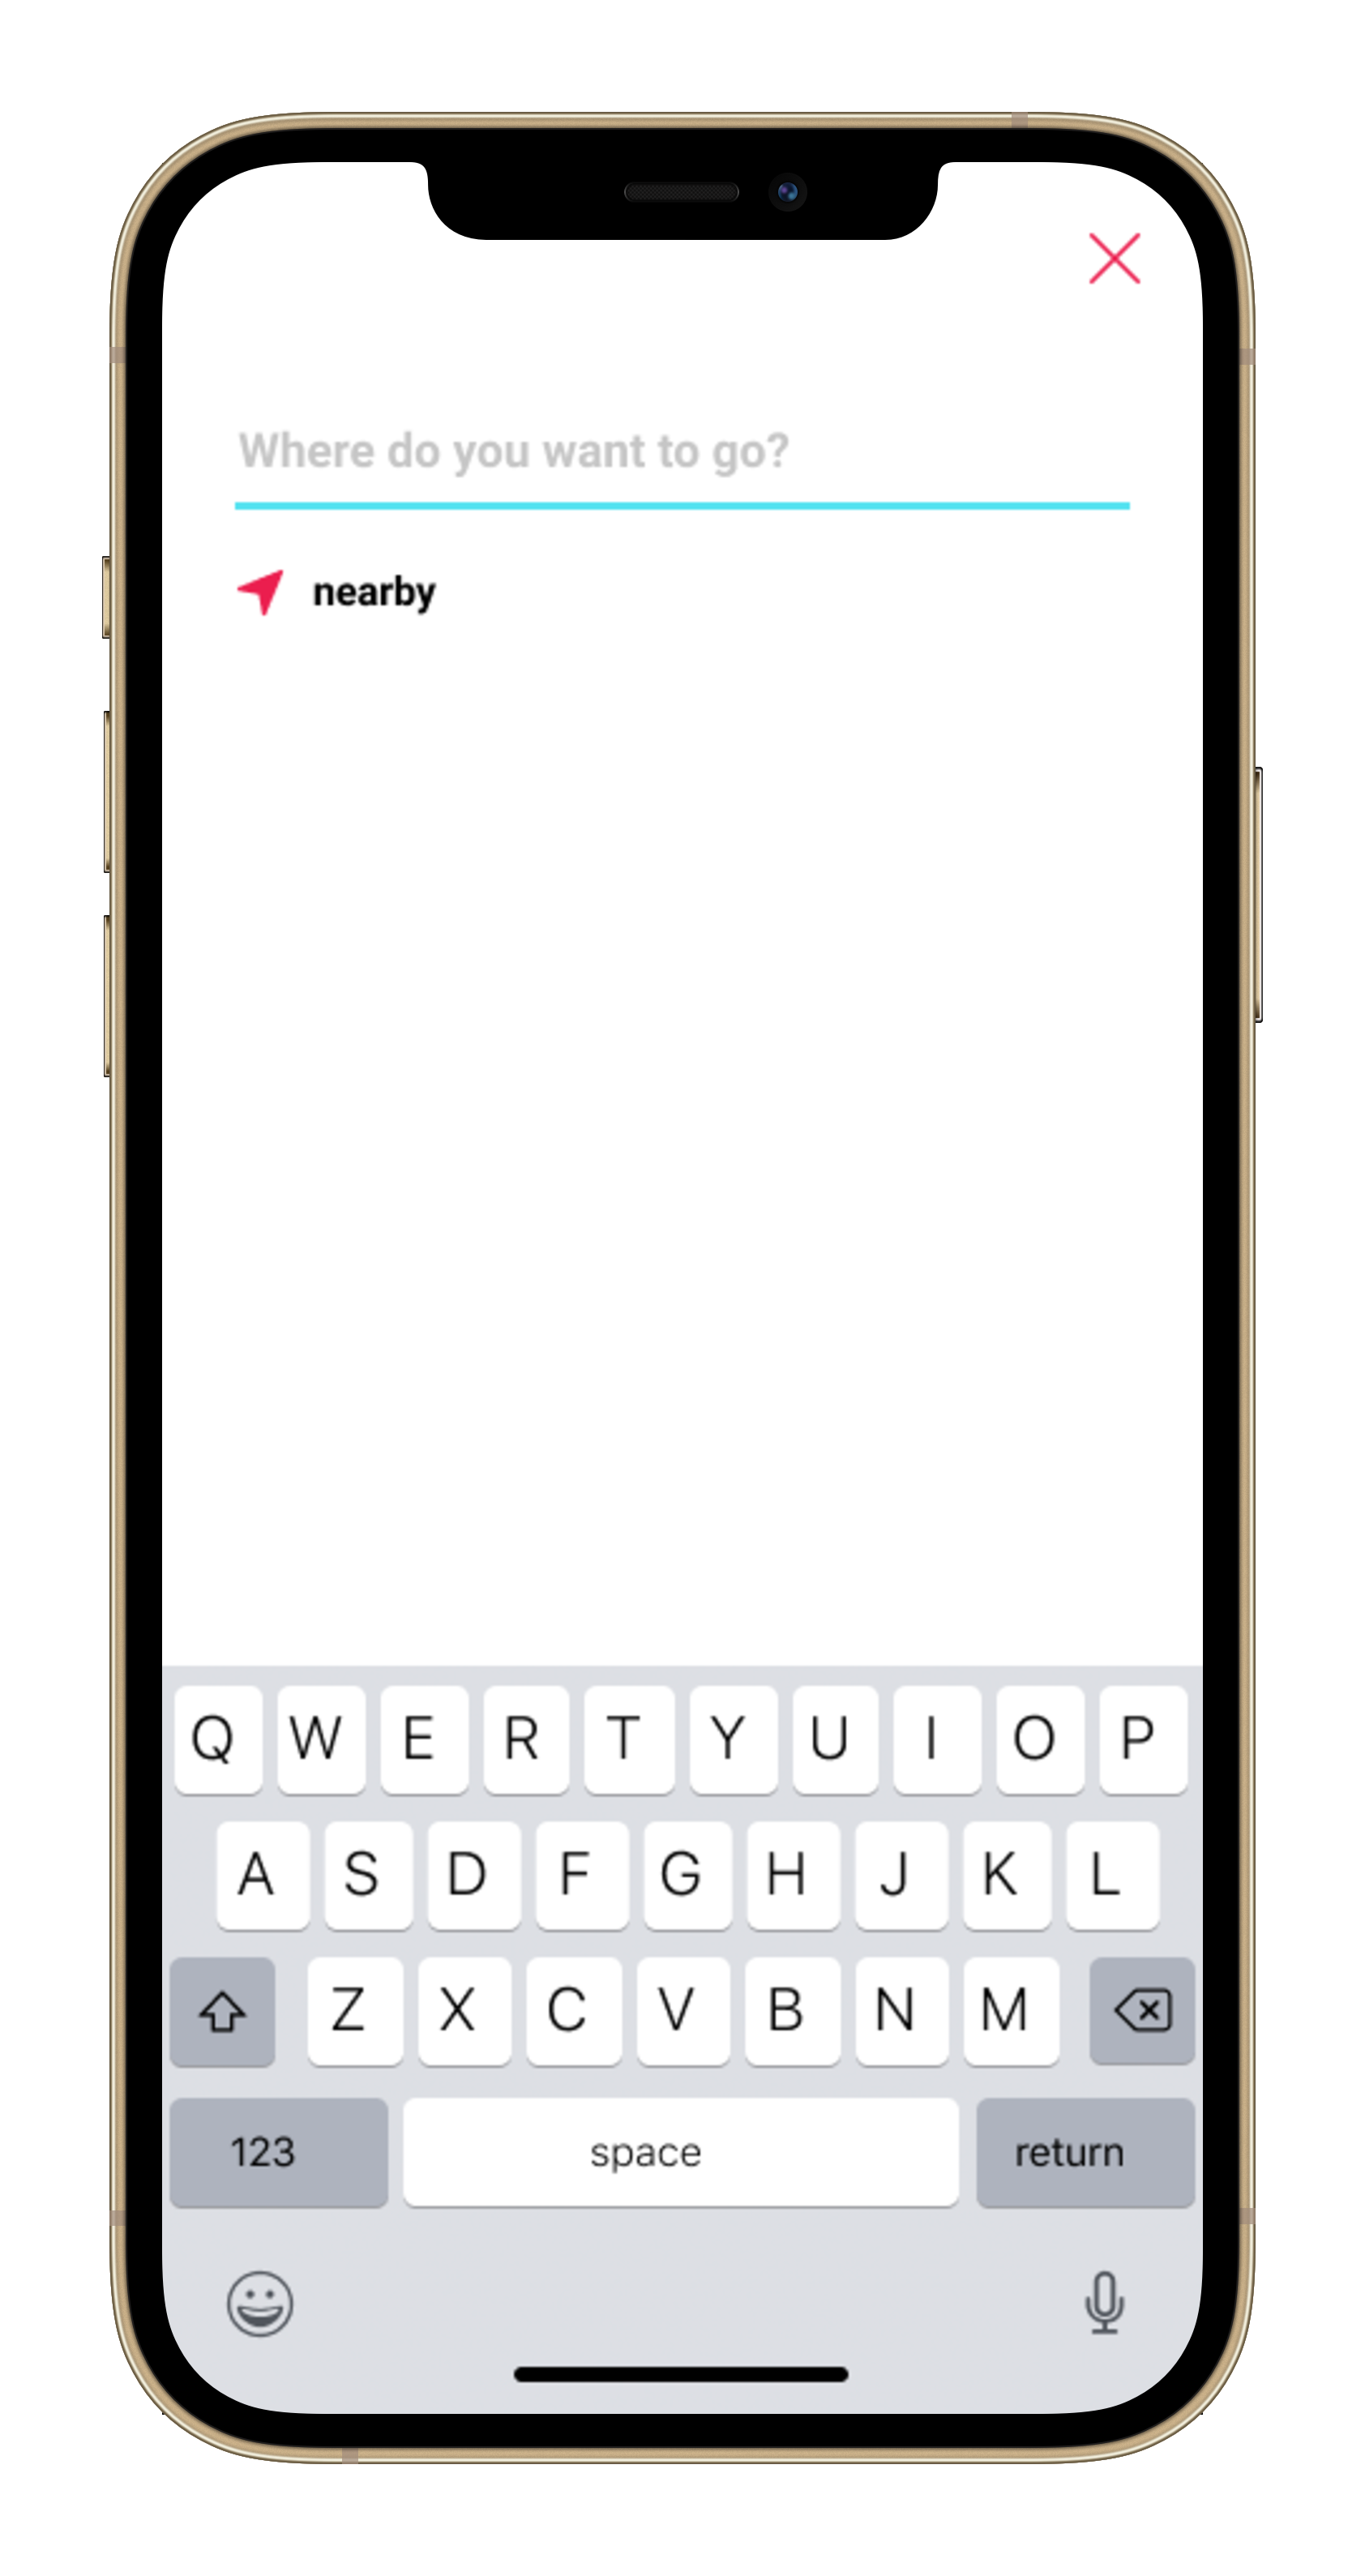
\includegraphics[width=0.9\textwidth]{Images/UserInterfaces/withiphonephrames/SearchPage_iphone12promaxgold_portrait.png}
    \caption{\label{fig:InterfacesDiagram}{Search Page Mockup}}
\end{minipage}
\hspace{.05\linewidth}
\begin{minipage}{.45\linewidth}
    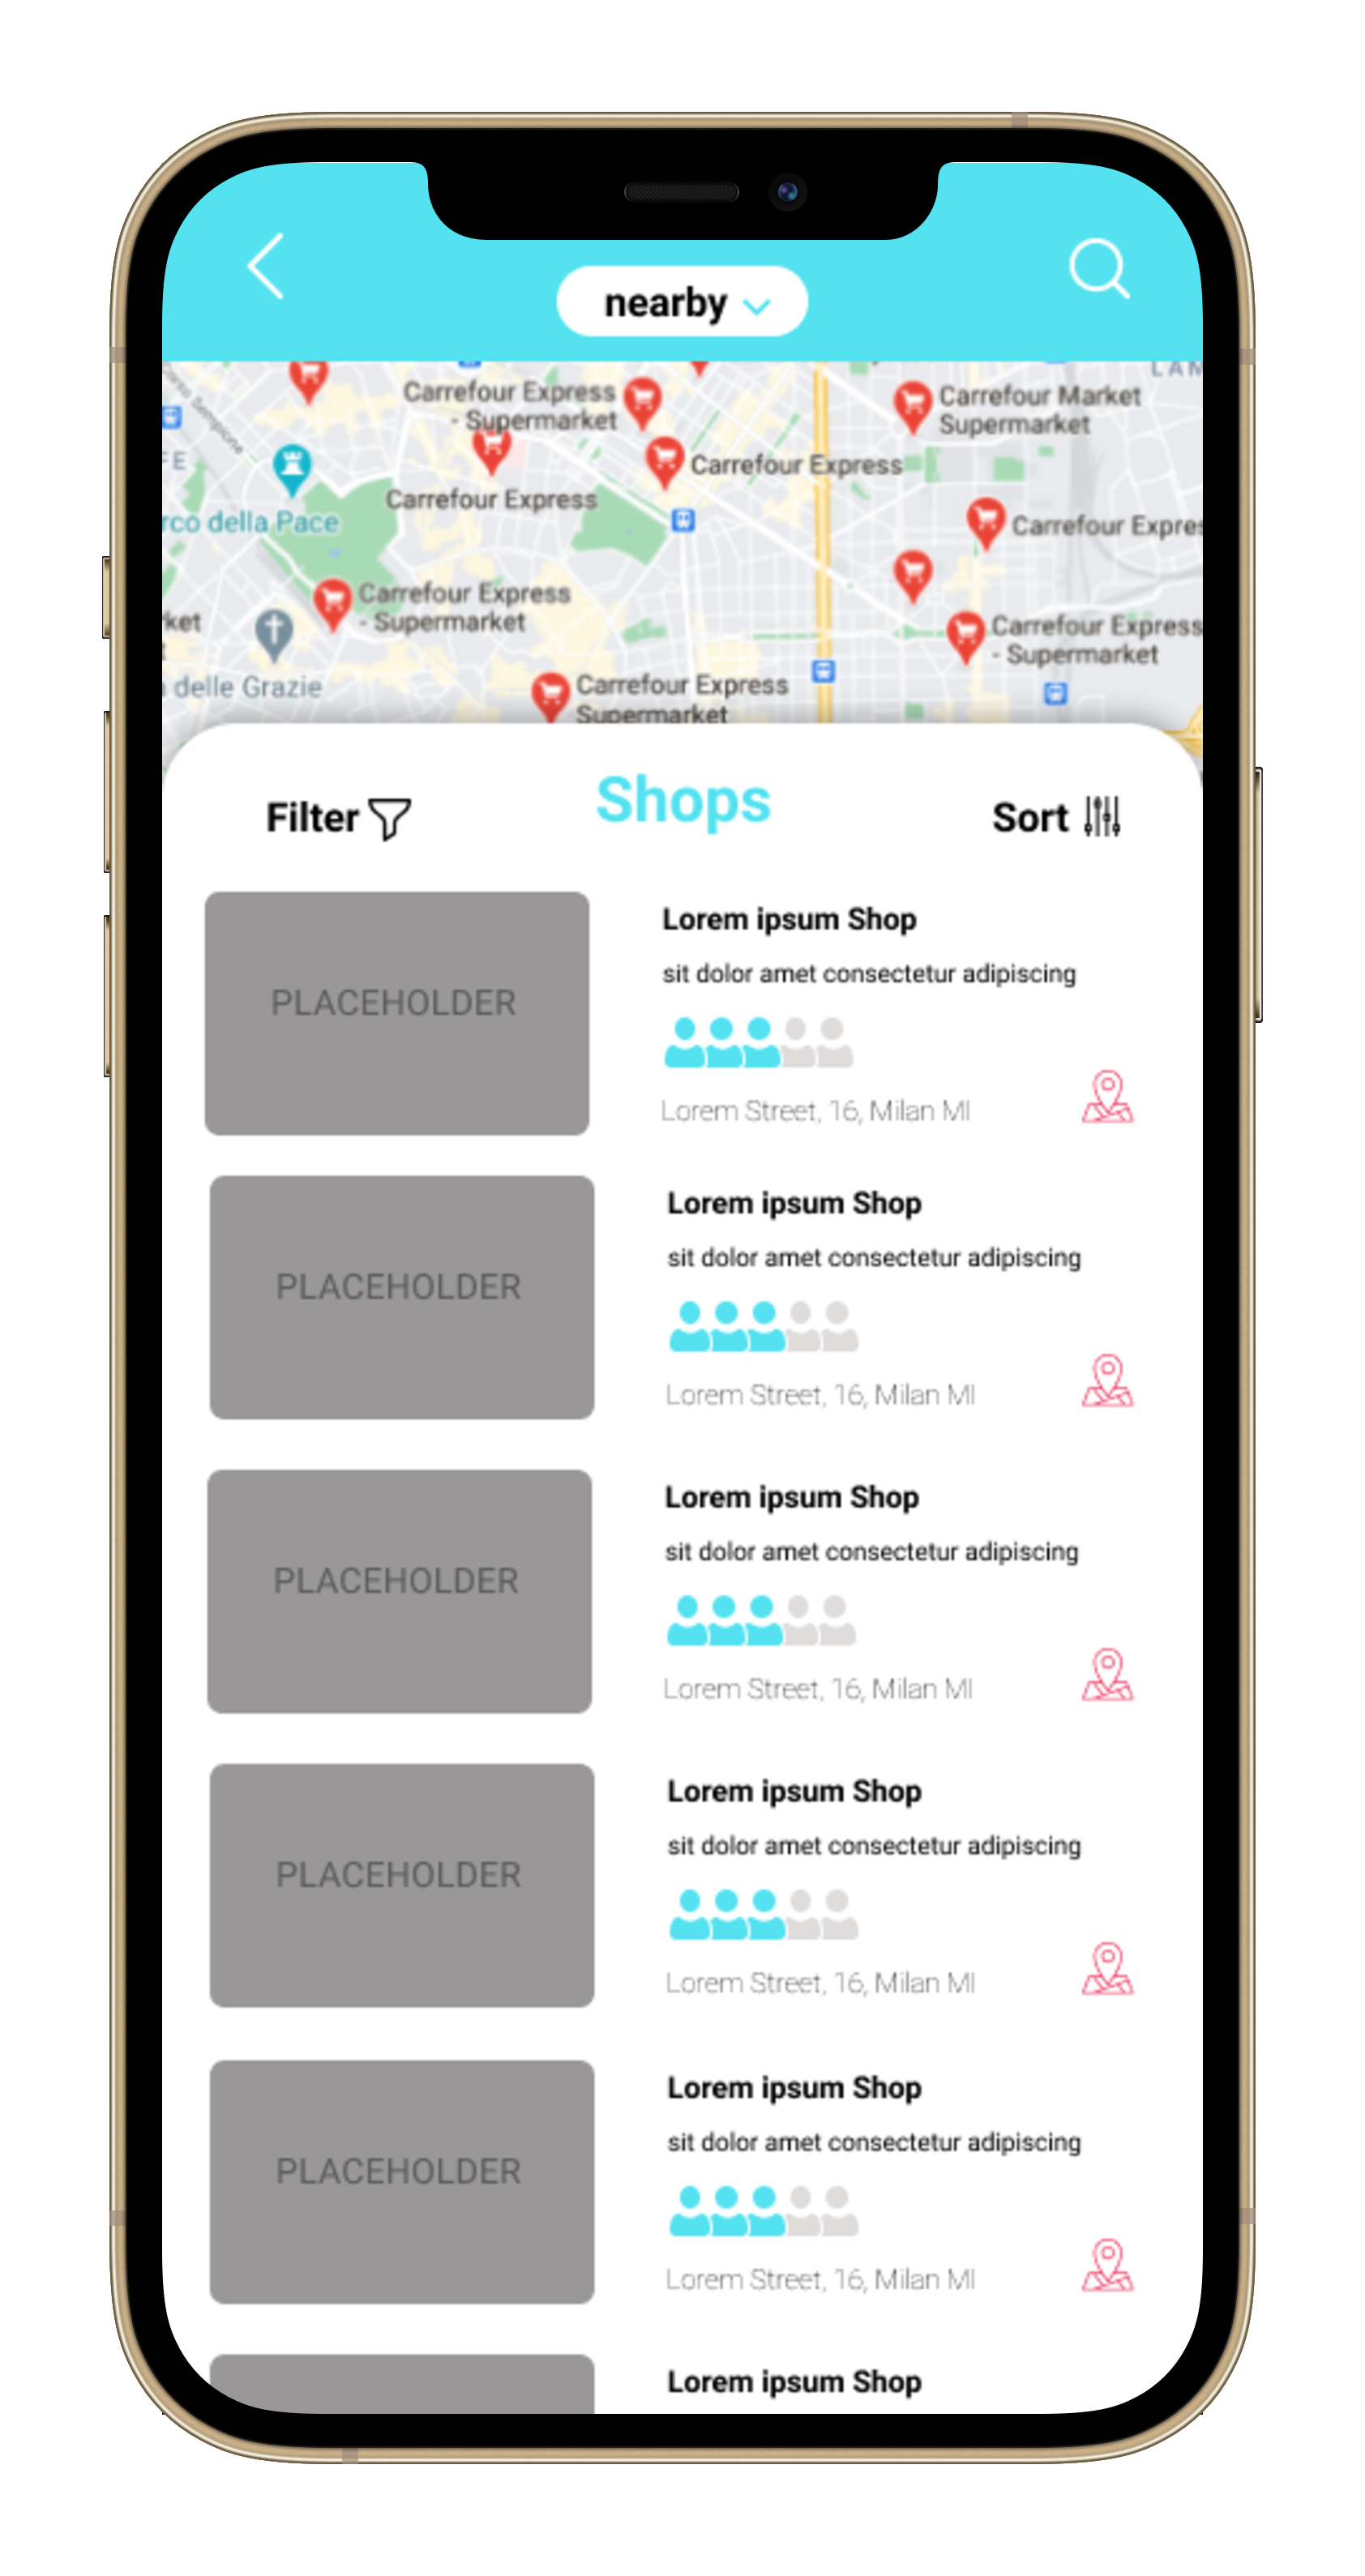
\includegraphics[width=0.9\textwidth]{Images/UserInterfaces/withiphonephrames/ShopsPage1_iphone12promaxgold_portrait.png}
    \caption{\label{fig:InterfacesDiagram}{Shops Page 1 Mockup}}
\end{minipage}
\end{figure}

\begin{figure}
    \centering
    \begin{minipage}{.45\linewidth}
    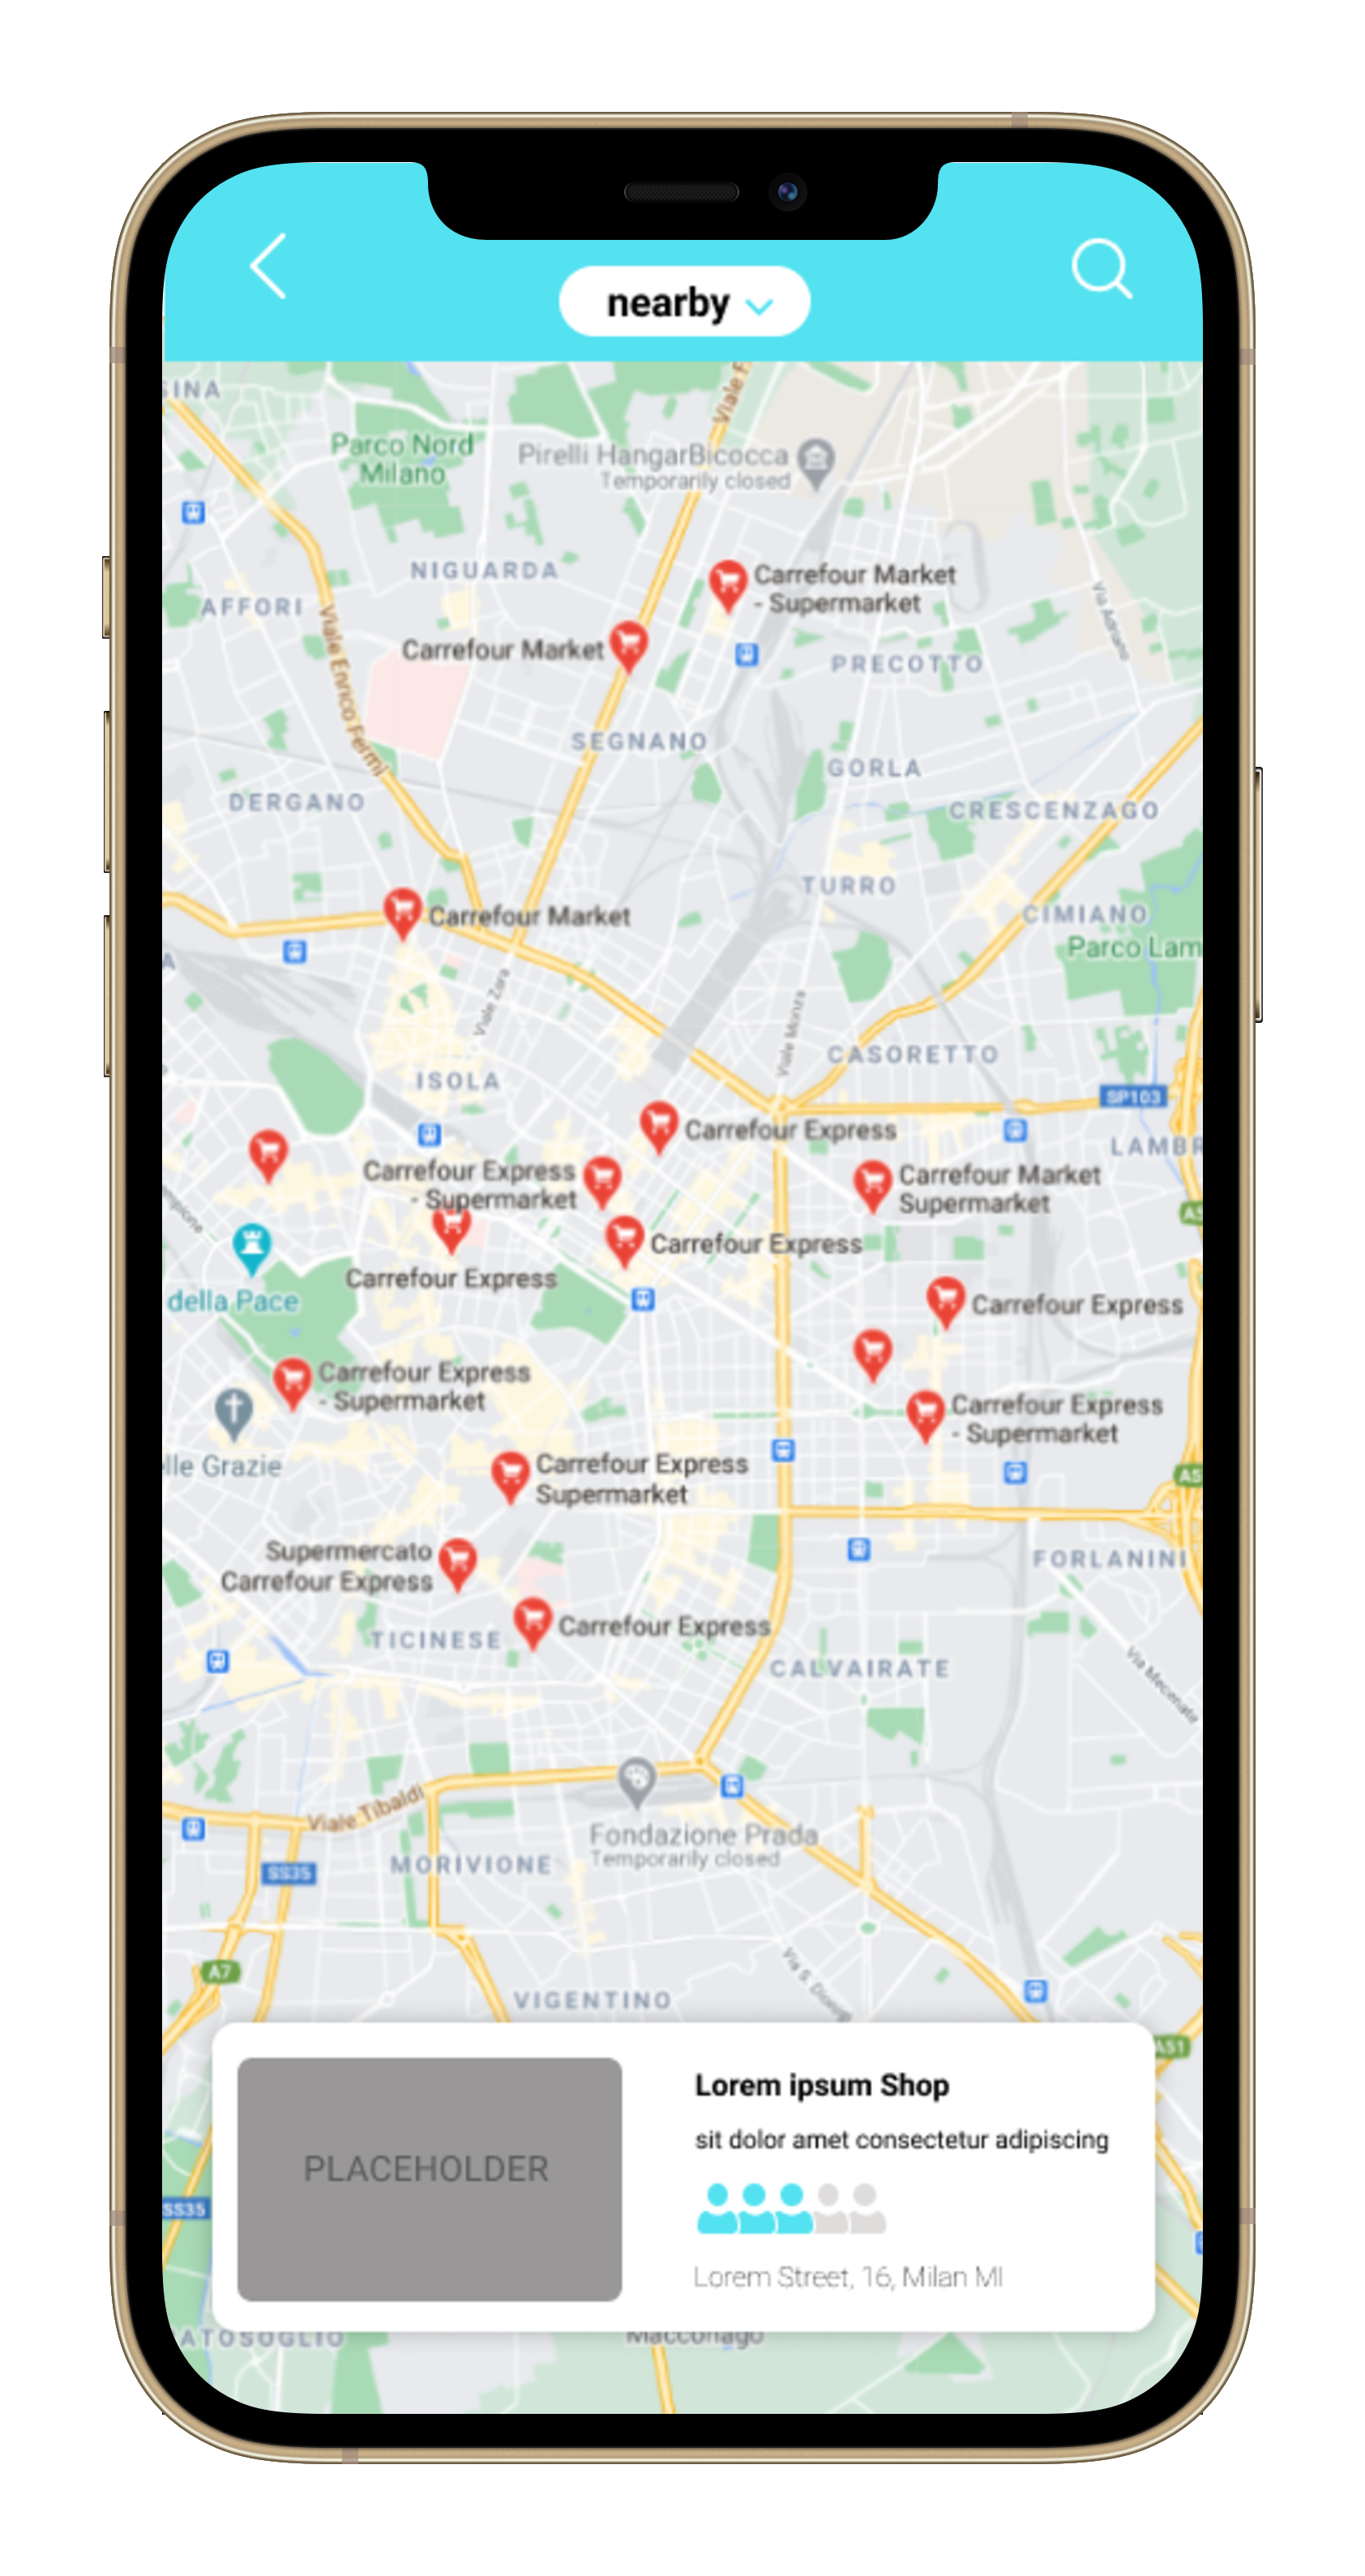
\includegraphics[width=0.9\textwidth]{Images/UserInterfaces/withiphonephrames/ShopsPage2_iphone12promaxgold_portrait.png}
    \caption{\label{fig:InterfacesDiagram}{Shops Page 2 Mockup}}
\end{minipage}
\hspace{.05\linewidth}
\begin{minipage}{.45\linewidth}
    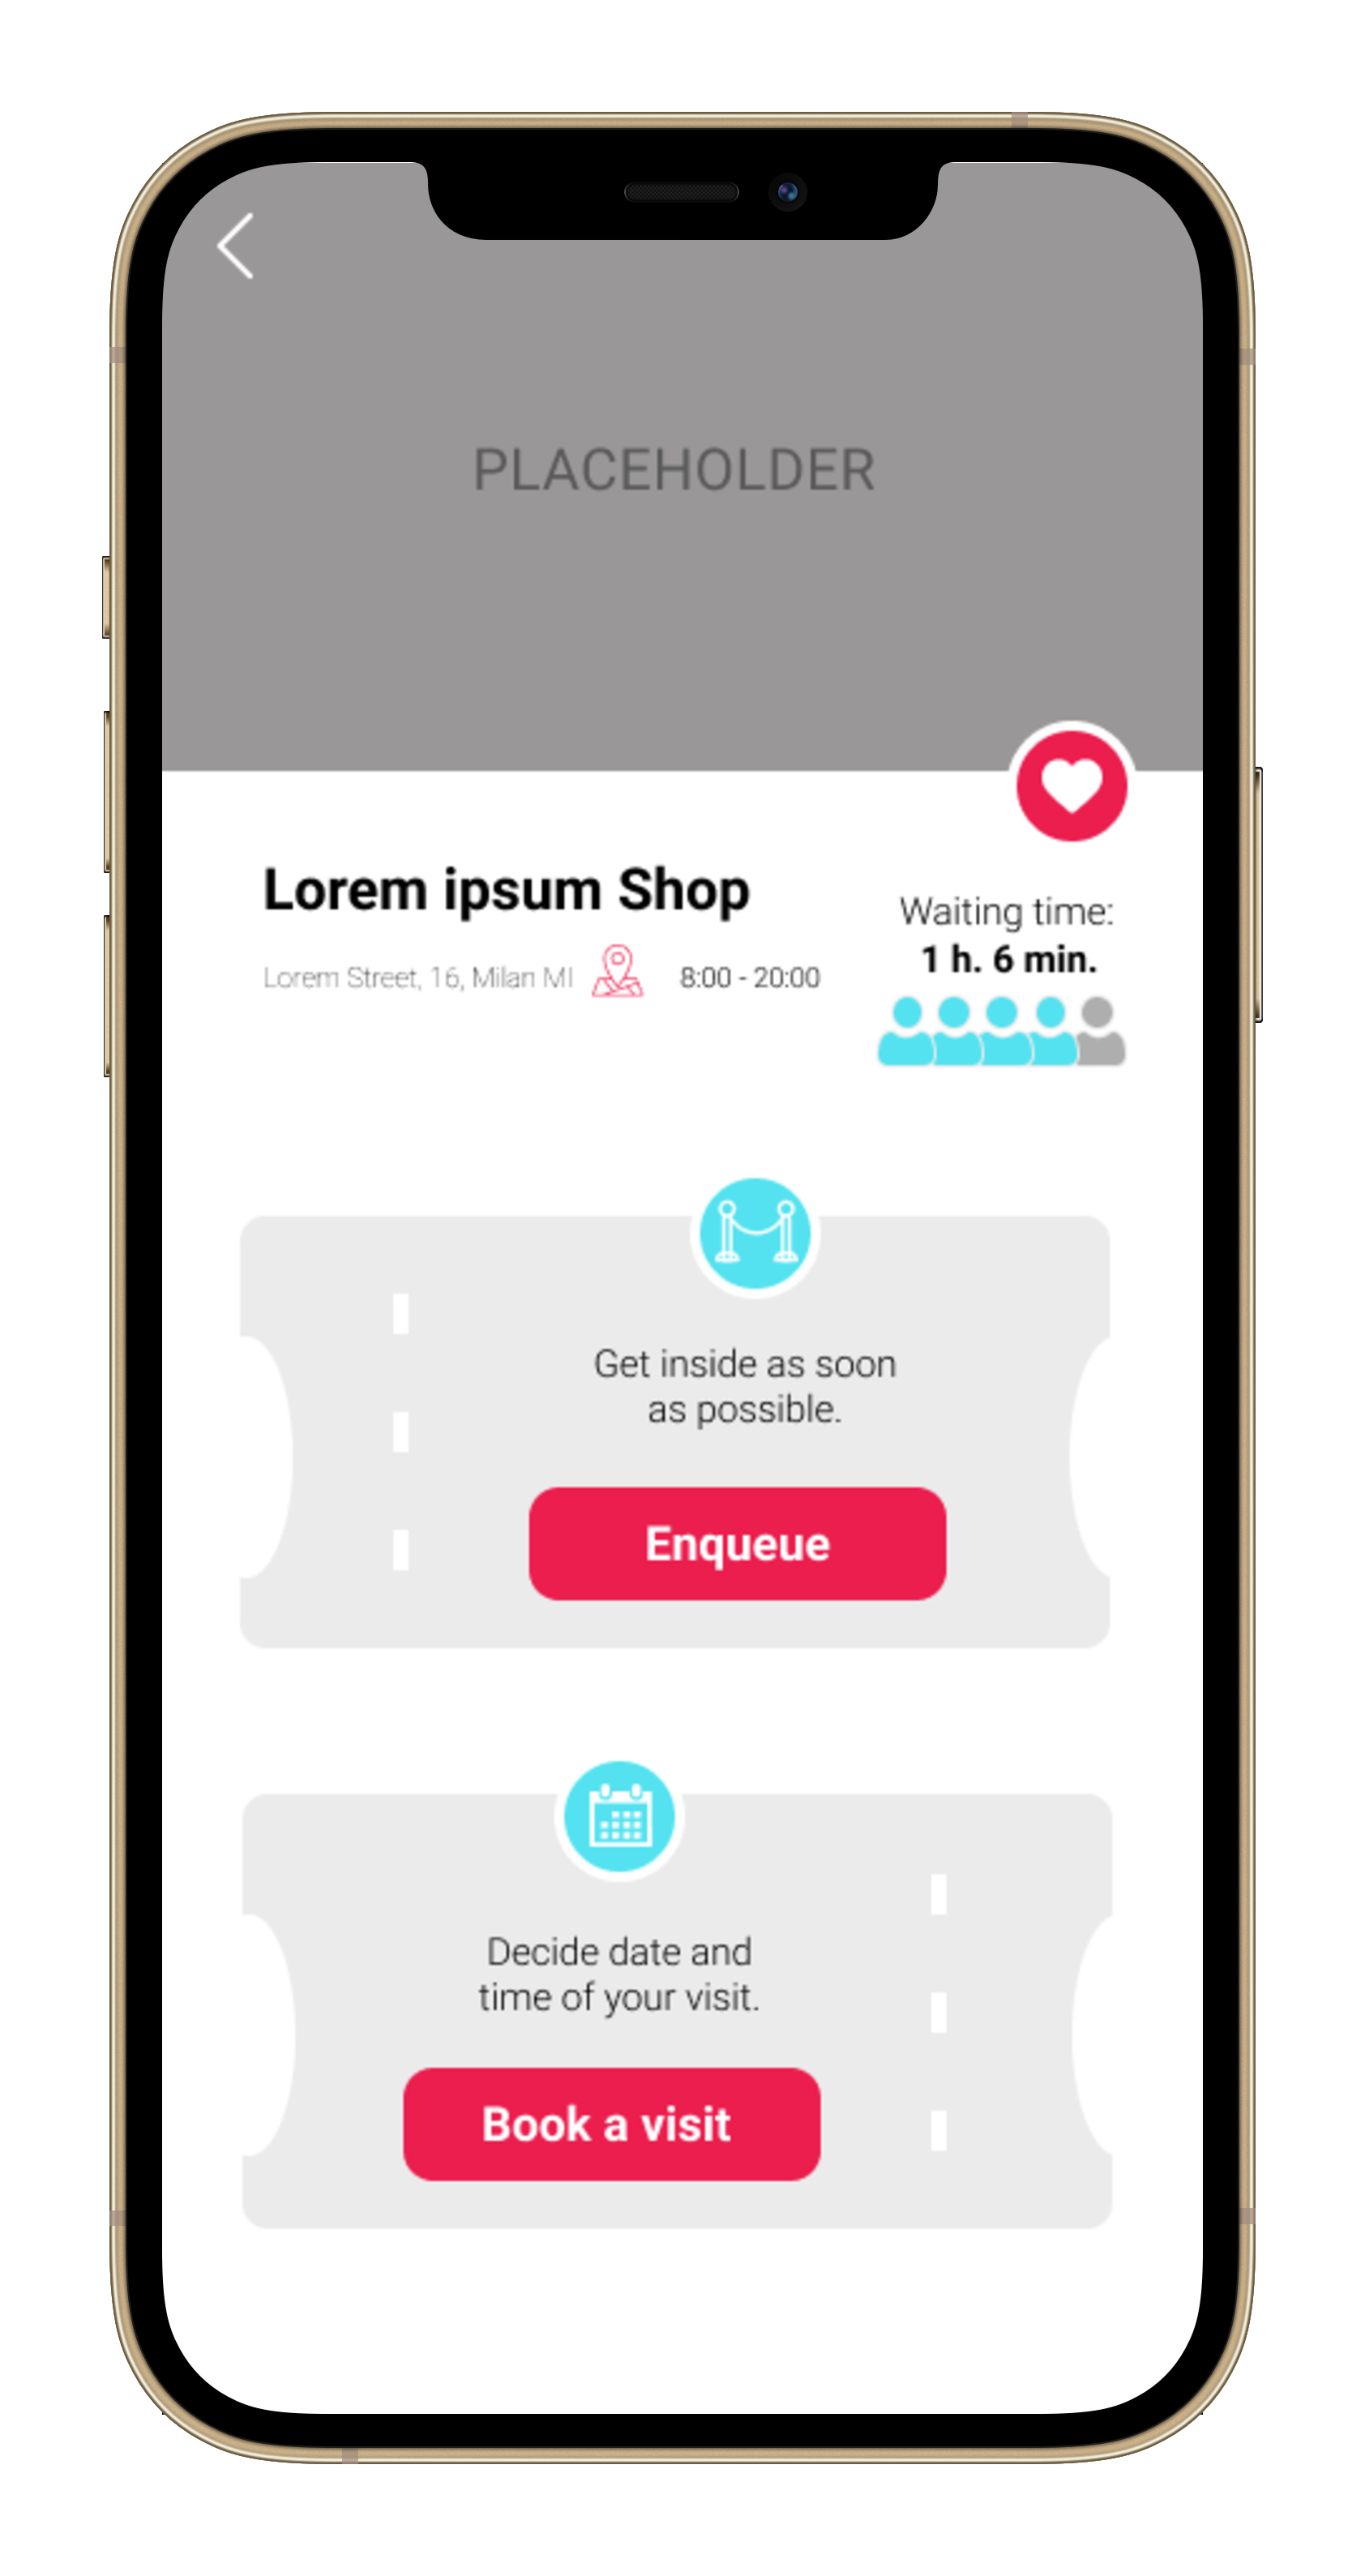
\includegraphics[width=0.9\textwidth]{Images/UserInterfaces/withiphonephrames/ShopPage_iphone12promaxgold_portrait.png}
    \caption{\label{fig:InterfacesDiagram}{Shop Page Mockup}}
\end{minipage}
\end{figure}

\begin{figure}
    \centering
    \begin{minipage}{.45\linewidth}
    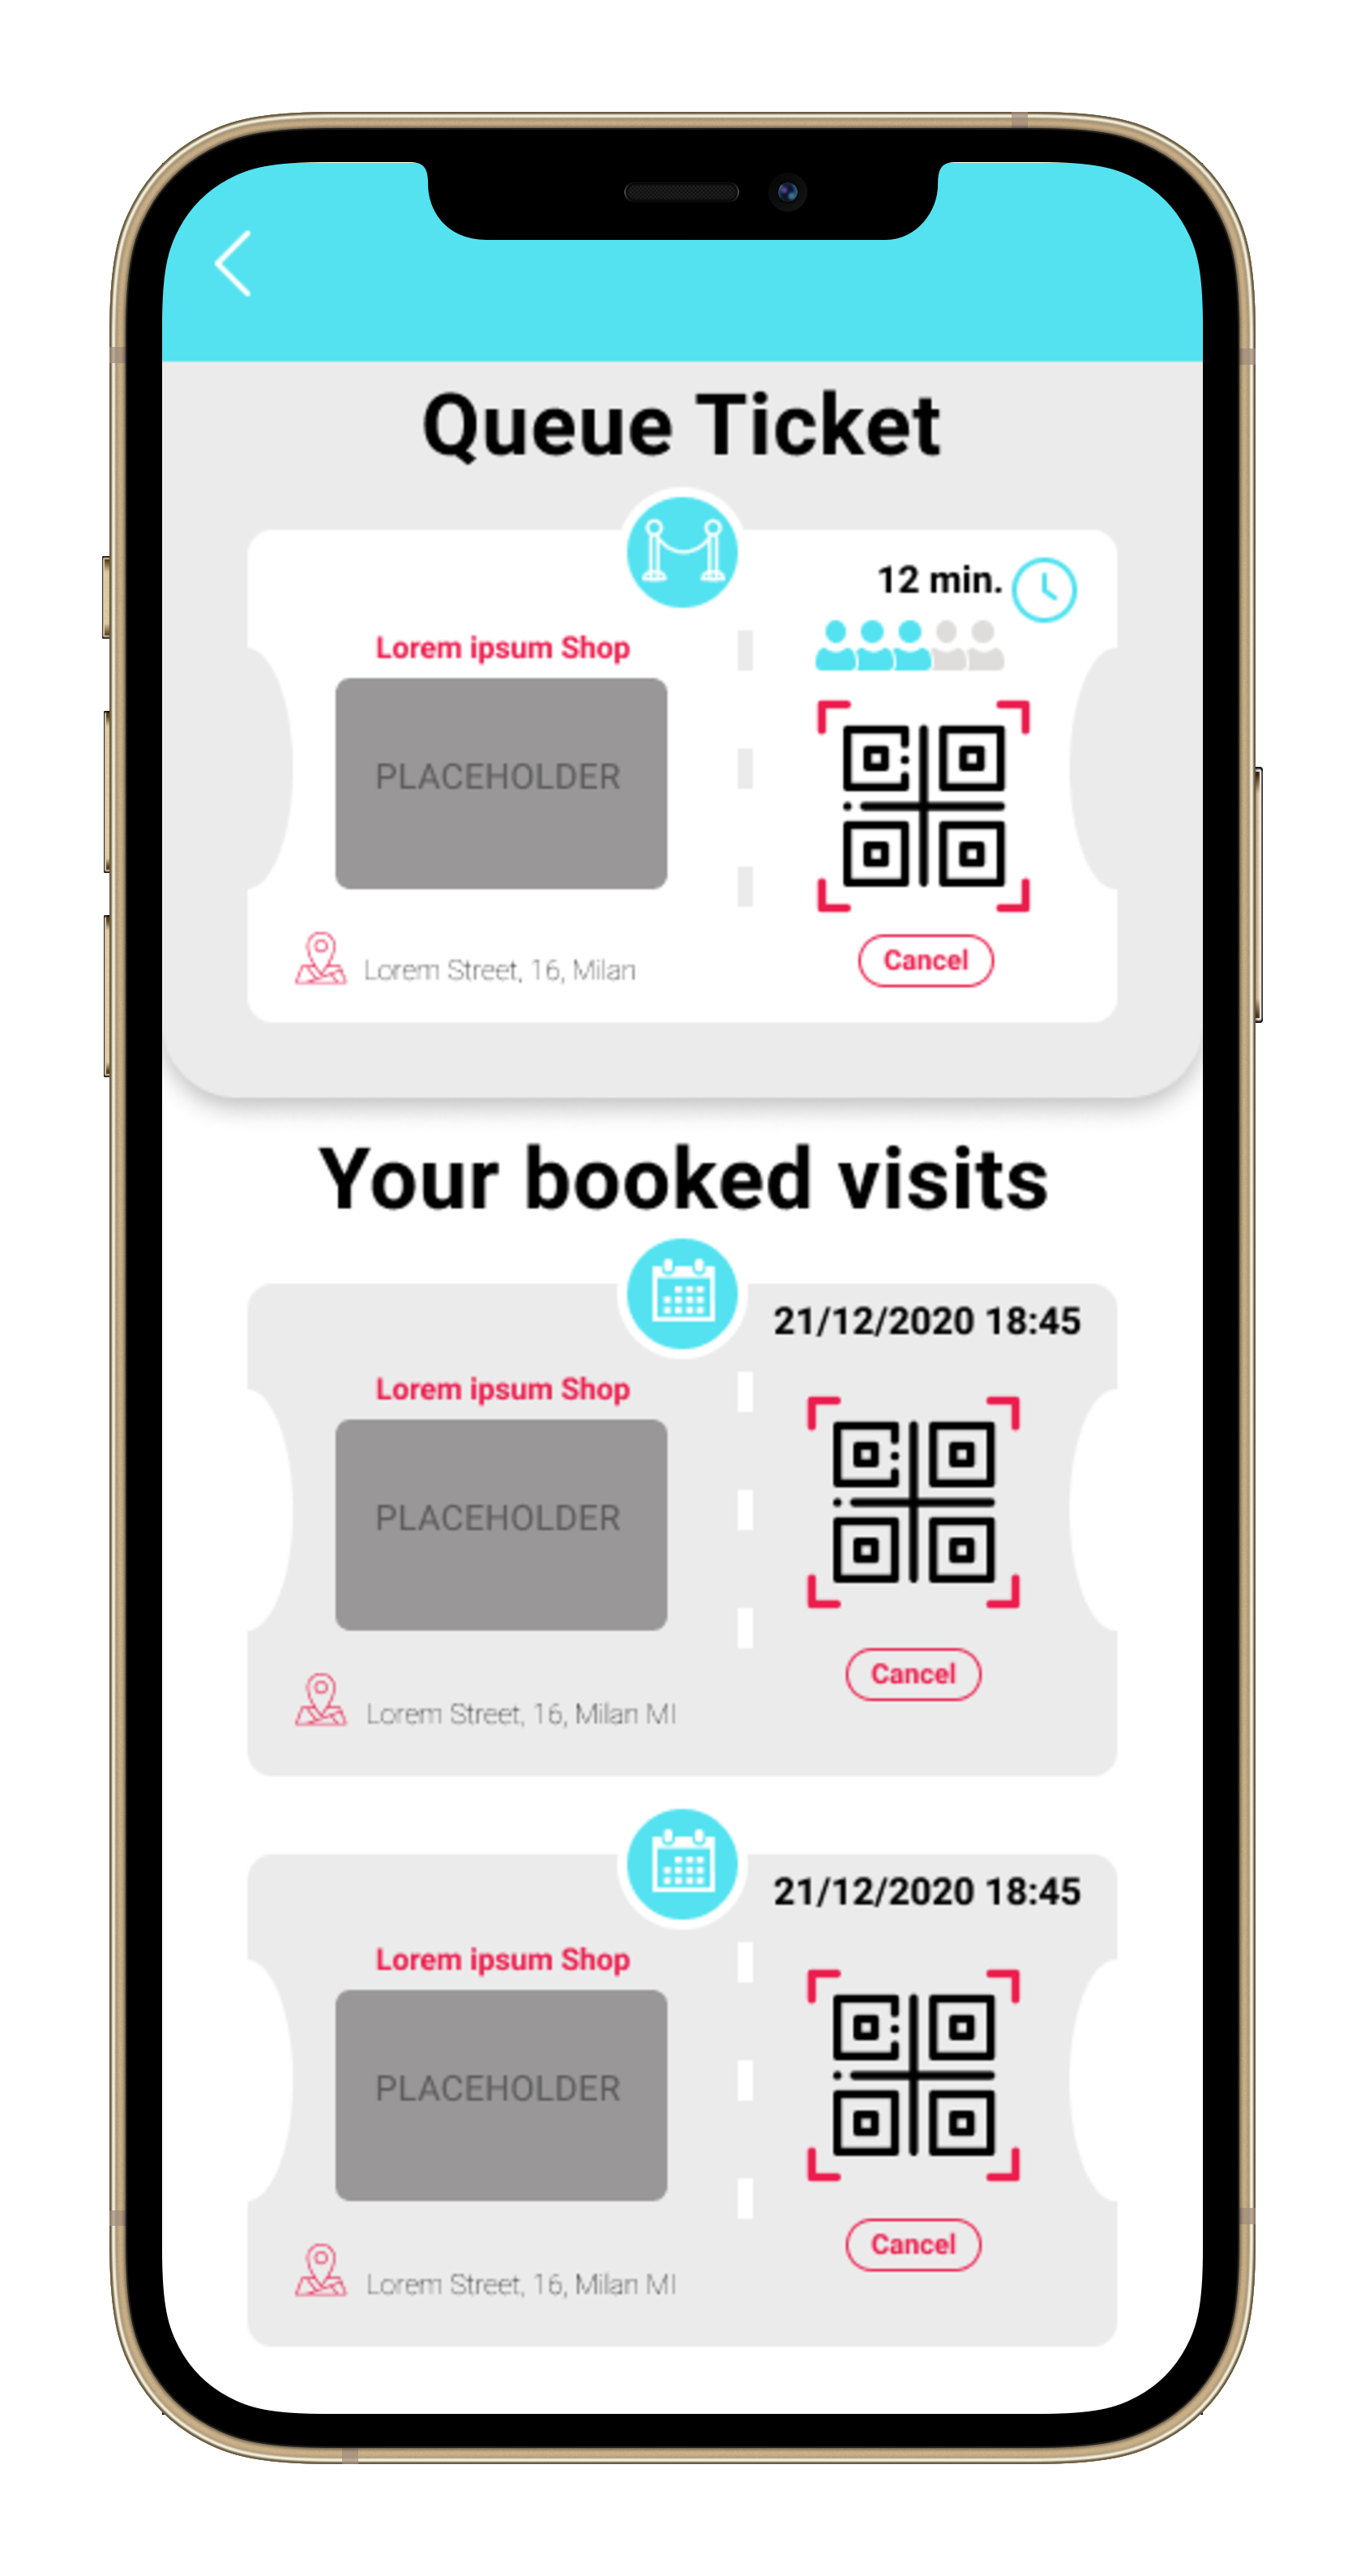
\includegraphics[width=0.9\textwidth]{Images/UserInterfaces/withiphonephrames/YourTicketPage_iphone12promaxgold_portrait.png}
    \caption{\label{fig:InterfacesDiagram}{Your Ticket Page Mockup}}
\end{minipage}
\hspace{.05\linewidth}
\begin{minipage}{.45\linewidth}
    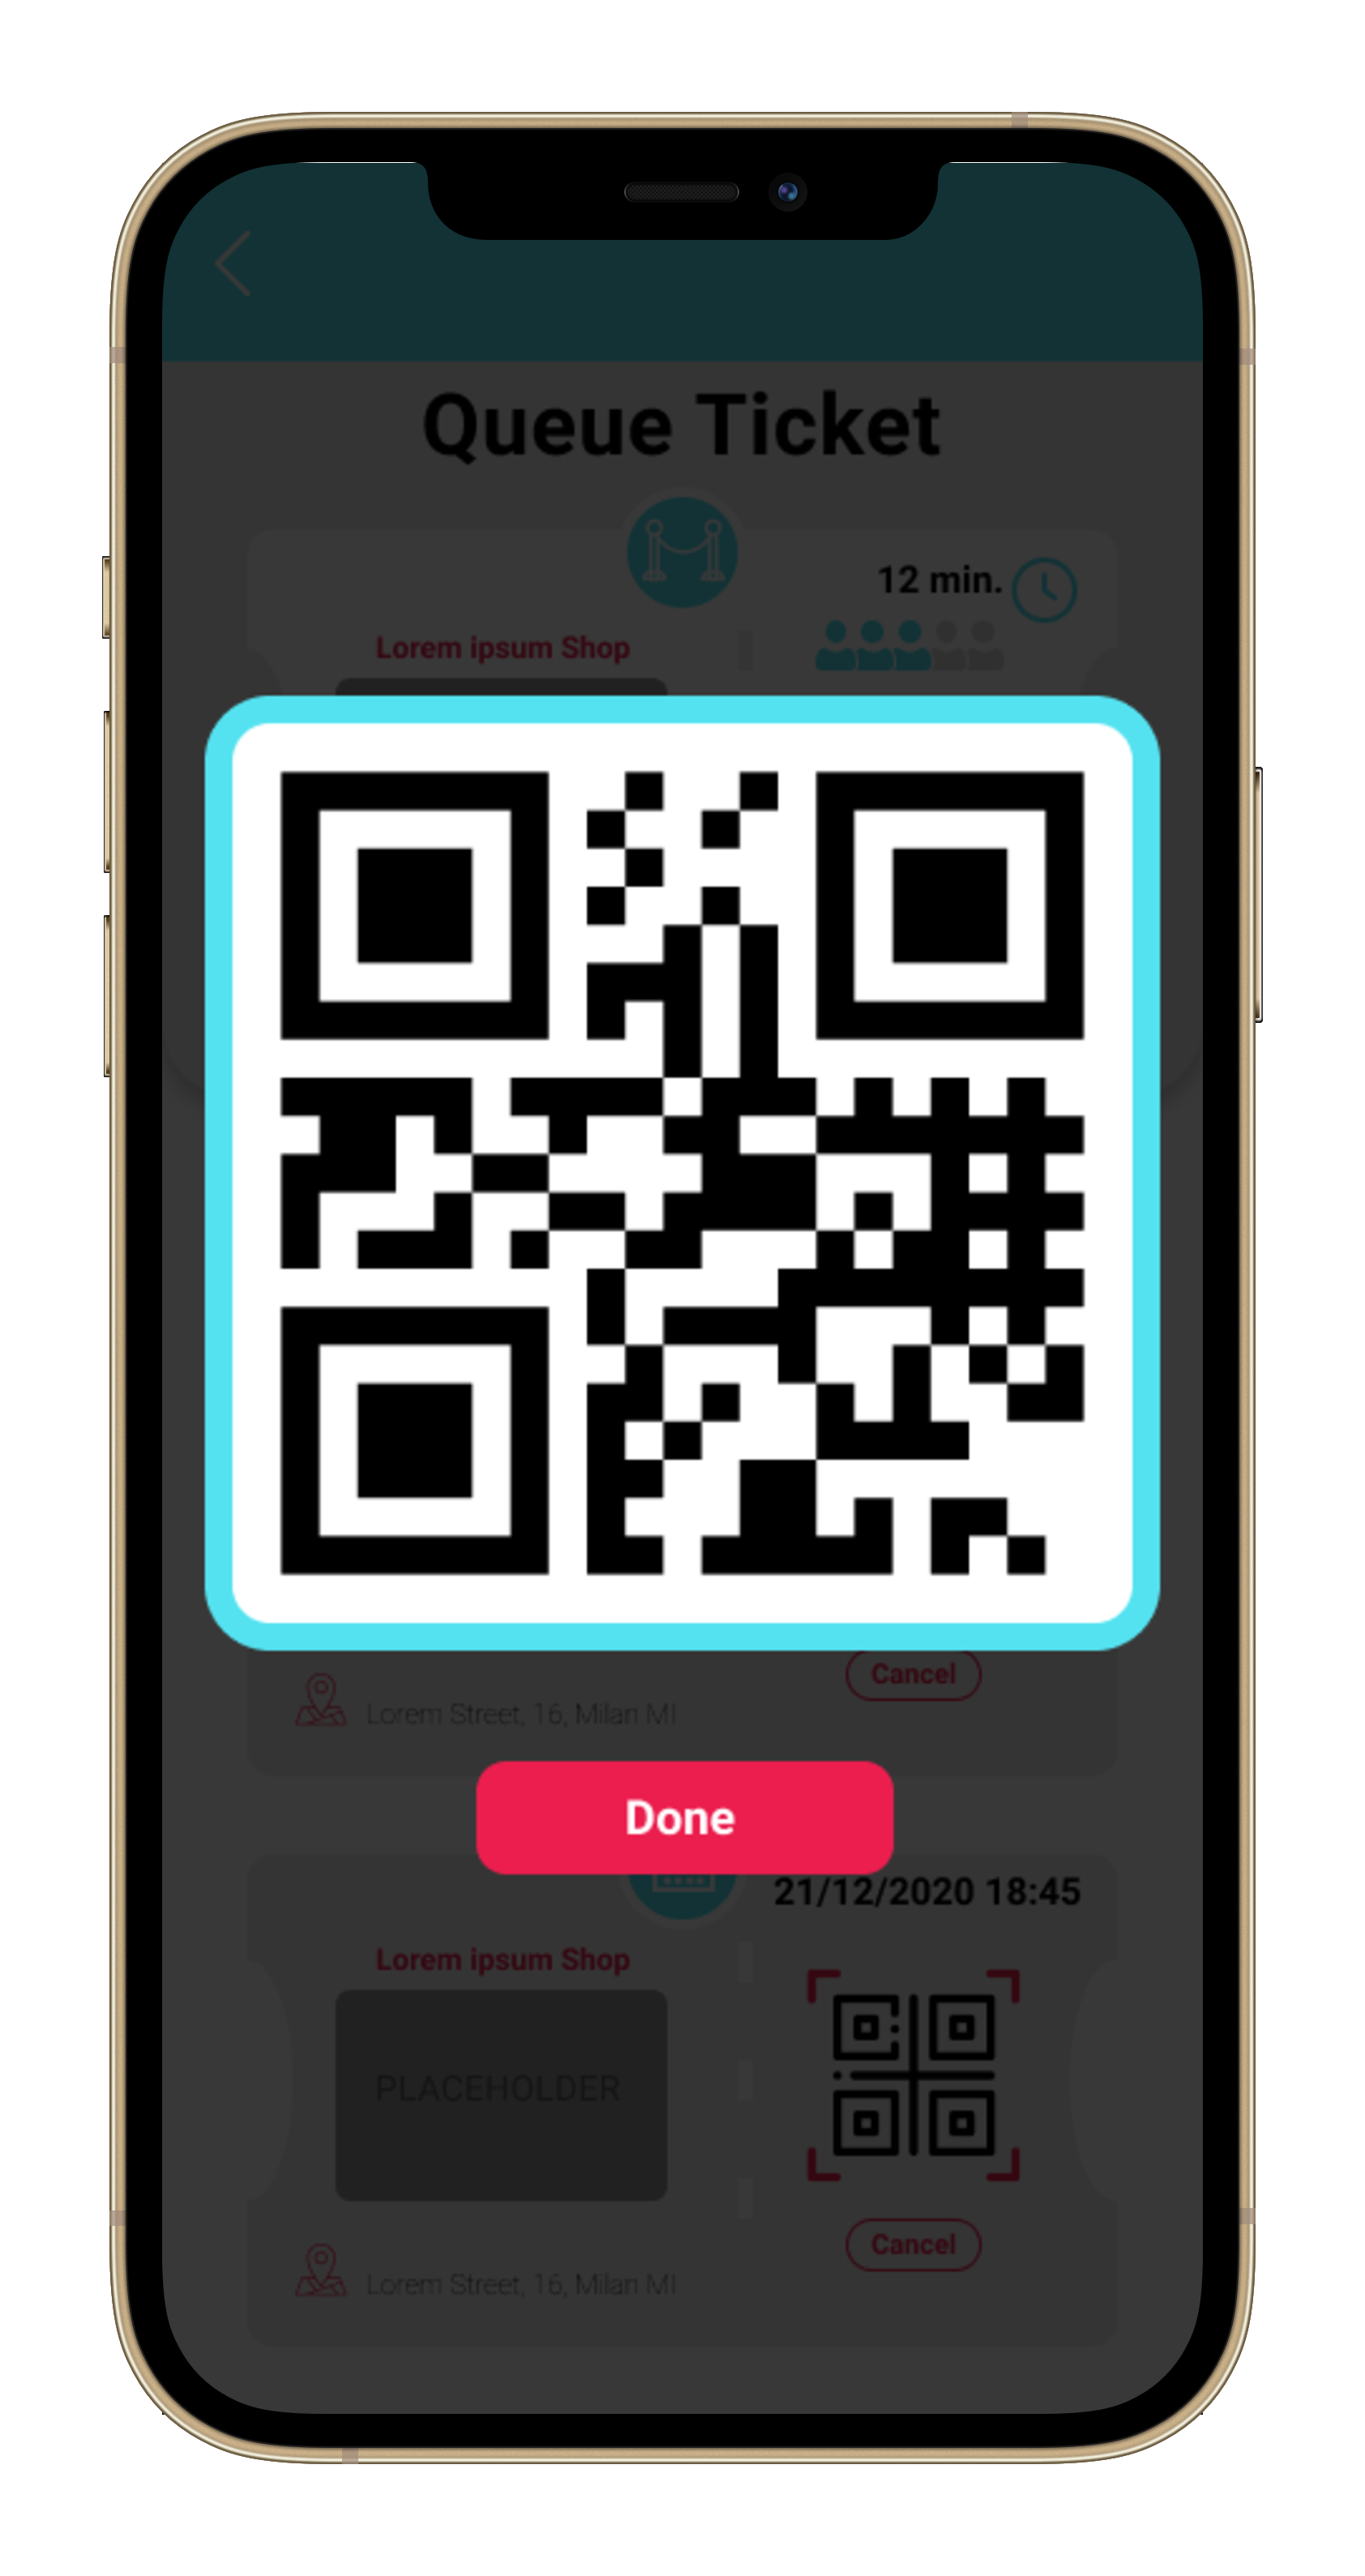
\includegraphics[width=0.9\textwidth]{Images/UserInterfaces/withiphonephrames/QRcodePage_iphone12promaxgold_portrait.png}
    \caption{\label{fig:InterfacesDiagram}{QR code Page Mockup}}
\end{minipage}
\end{figure}

\begin{figure}[h!]
    \centering
    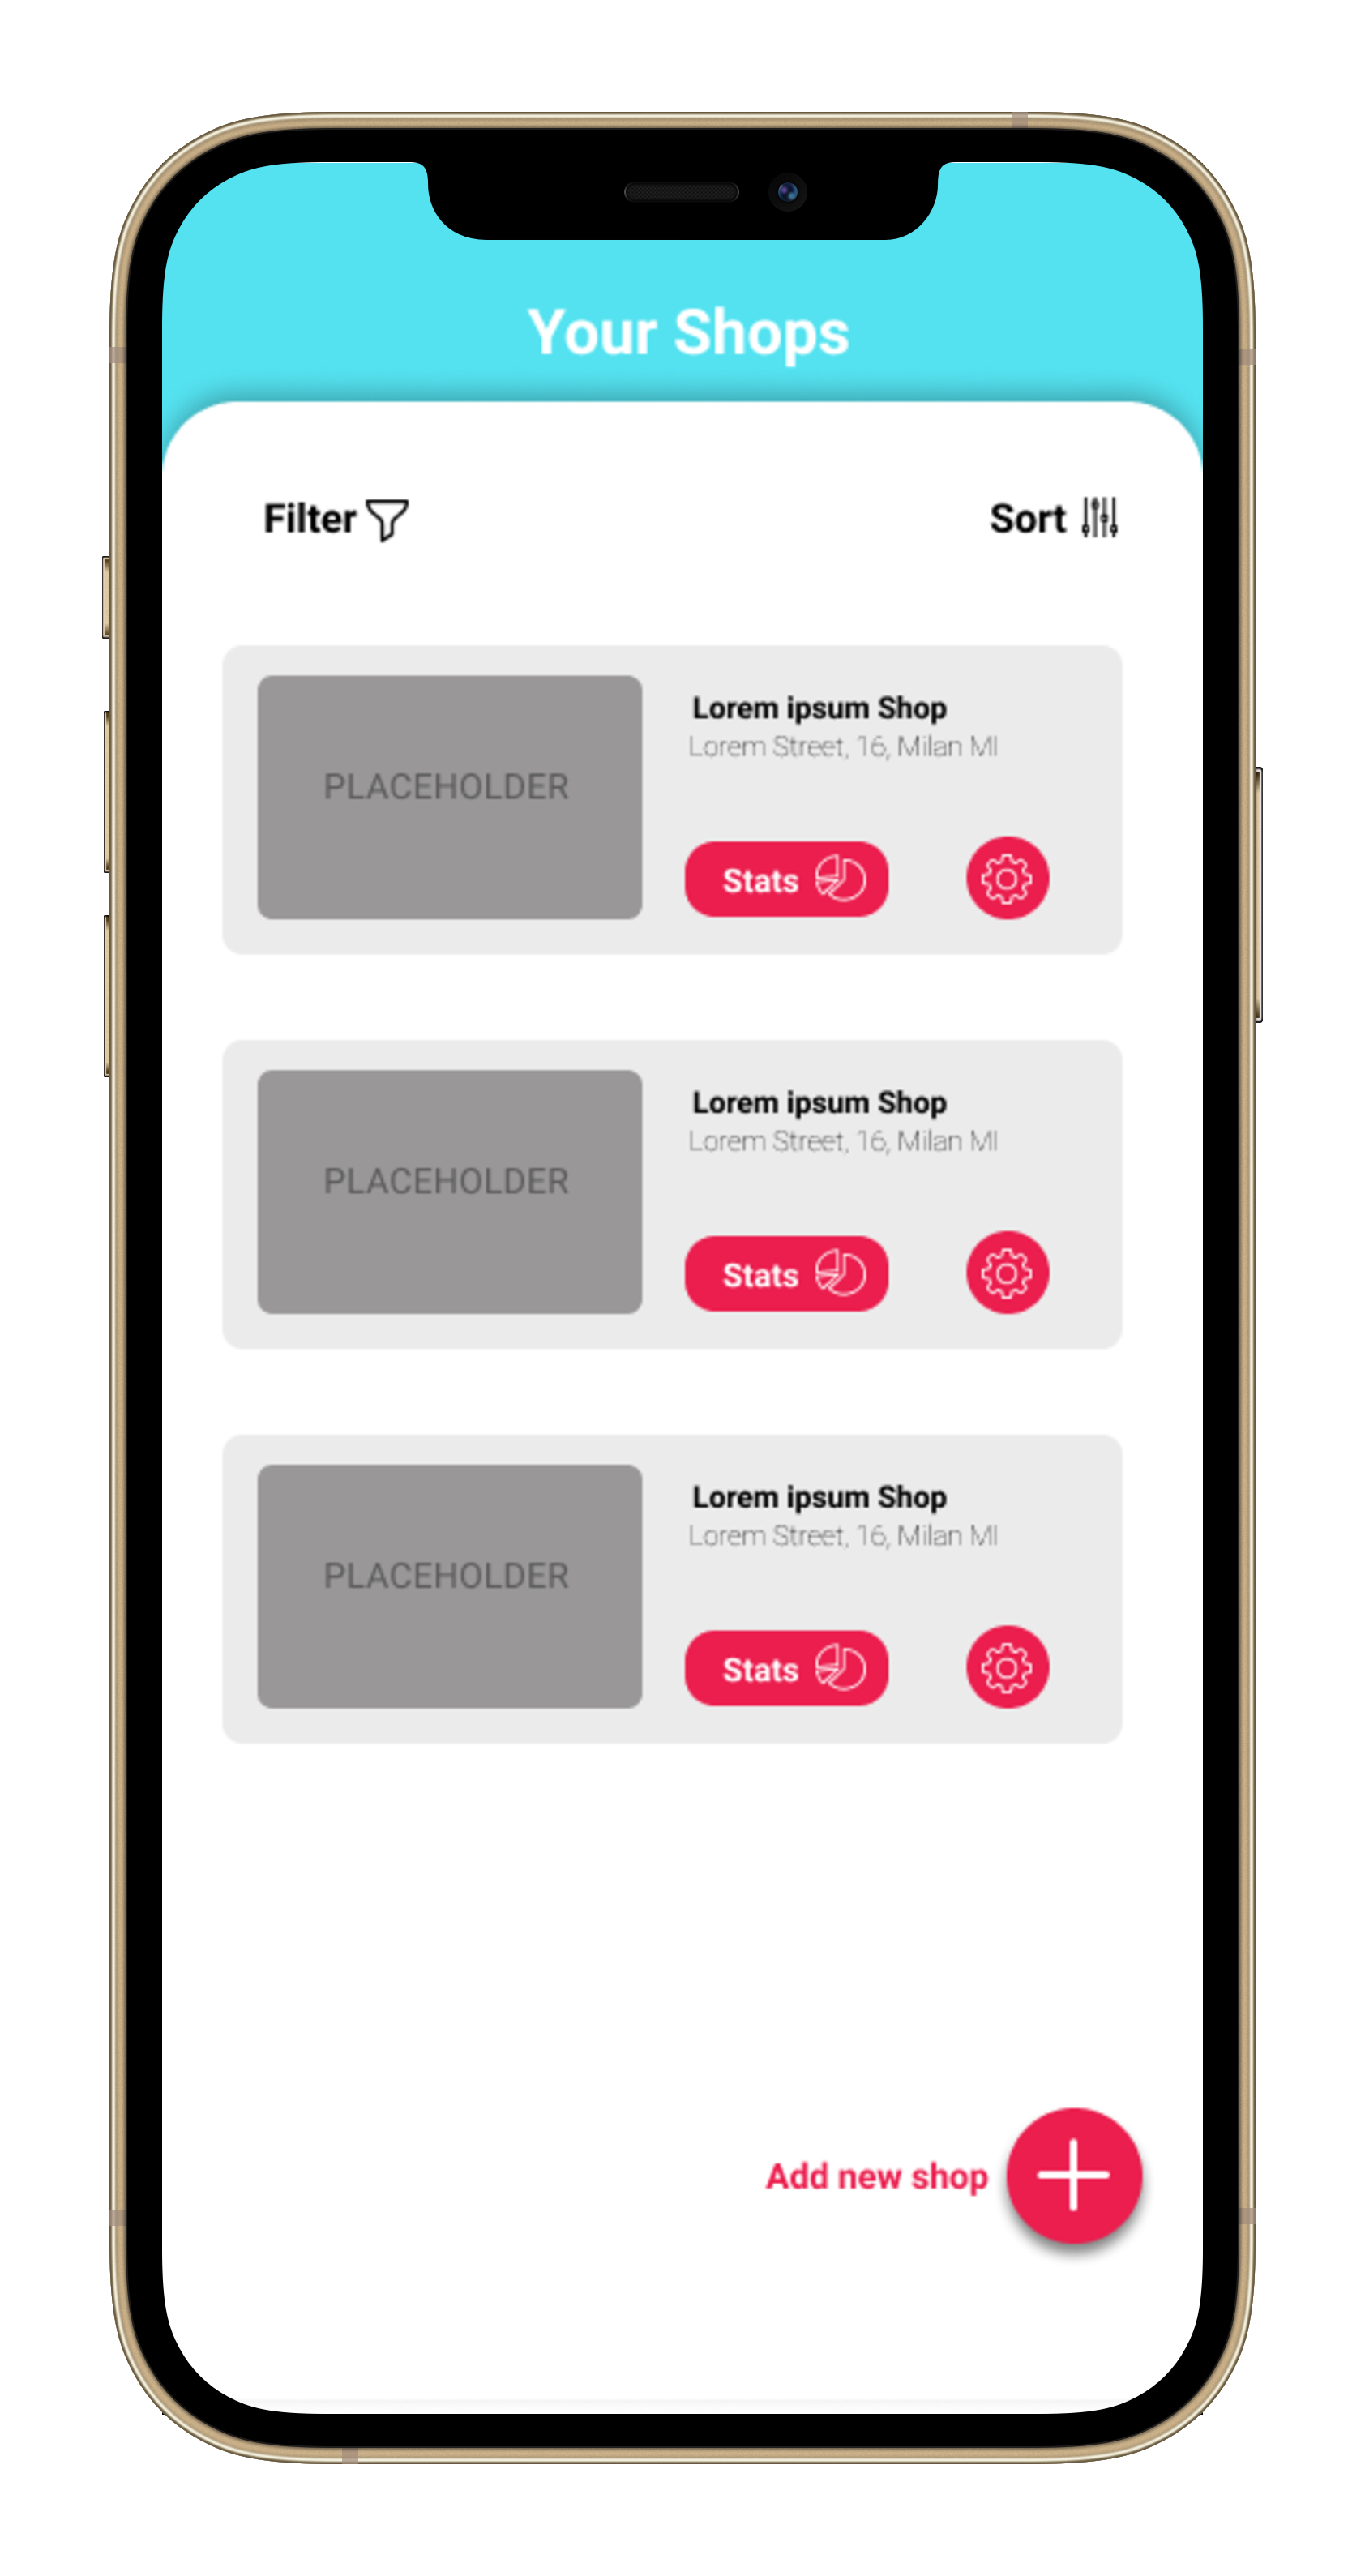
\includegraphics[width=0.405\textwidth]{Images/UserInterfaces/withiphonephrames/ManagerHomePage_iphone12promaxgold_portrait.png}
    \caption{\label{fig:InterfacesDiagram}{Manager Home Page Mockup}}
\end{figure}